% GA4GH File Encryption Standard specification
% When editing, please start all sentences on a new line; and try to avoid source lines longer than 120 characters.
\documentclass[10pt]{article}
\usepackage[numbib]{tocbibind}
\usepackage{titlesec}
\newcommand{\sectionbreak}{\clearpage}
\usepackage[margin=1in]{geometry}
\usepackage{parskip}
\usepackage{algpseudocode}
\usepackage{draftwatermark}
\usepackage{tikz}
\usetikzlibrary{positioning,shapes.multipart}
\usepackage[pdfborder={0 0 0},hyperfootnotes=false]{hyperref}
\newcommand{\mailtourl}[1]{\href{mailto:#1}{\tt #1}}
\newcommand{\tagvalue}[1]{\tt #1}
\newcommand{\tagregex}[1]{\tt #1}
\newcommand{\kw}[1]{\texttt{#1}}
\newlength{\maxwidth}
\newcommand{\algalign}[2] % #1 = text to left, #2 = text to right
{\makebox[\maxwidth][l]{$#1{}$}${}#2$}

\SetWatermarkAngle{315}
\SetWatermarkText{PRELIMINARY}
\SetWatermarkScale{4}

\begin{document}

% GA4GH File Encryption Standard specification
% When editing, please start all sentences on a new line; and try to avoid source lines longer than 120 characters.
\documentclass[10pt]{article}
\usepackage[numbib]{tocbibind}
\usepackage{titlesec}
\newcommand{\sectionbreak}{\clearpage}
\usepackage[margin=1in]{geometry}
\usepackage{parskip}
\usepackage{algpseudocode}
\usepackage{tikz}
\usetikzlibrary{positioning,shapes.multipart}
\usepackage[pdfborder={0 0 0},hyperfootnotes=false]{hyperref}
\newcommand{\mailtourl}[1]{\href{mailto:#1}{\tt #1}}
\newcommand{\tagvalue}[1]{\tt #1}
\newcommand{\tagregex}[1]{\tt #1}
\newcommand{\kw}[1]{\texttt{#1}}
\newlength{\maxwidth}
\newcommand{\algalign}[2] % #1 = text to left, #2 = text to right
{\makebox[\maxwidth][l]{$#1{}$}${}#2$}

\begin{document}

% GA4GH File Encryption Standard specification
% When editing, please start all sentences on a new line; and try to avoid source lines longer than 120 characters.
\documentclass[10pt]{article}
\usepackage[numbib]{tocbibind}
\usepackage{titlesec}
\newcommand{\sectionbreak}{\clearpage}
\usepackage[margin=1in]{geometry}
\usepackage{parskip}
\usepackage{algpseudocode}
\usepackage{tikz}
\usetikzlibrary{positioning,shapes.multipart}
\usepackage[pdfborder={0 0 0},hyperfootnotes=false]{hyperref}
\newcommand{\mailtourl}[1]{\href{mailto:#1}{\tt #1}}
\newcommand{\tagvalue}[1]{\tt #1}
\newcommand{\tagregex}[1]{\tt #1}
\newcommand{\kw}[1]{\texttt{#1}}
\newlength{\maxwidth}
\newcommand{\algalign}[2] % #1 = text to left, #2 = text to right
{\makebox[\maxwidth][l]{$#1{}$}${}#2$}

\begin{document}

% GA4GH File Encryption Standard specification
% When editing, please start all sentences on a new line; and try to avoid source lines longer than 120 characters.
\documentclass[10pt]{article}
\usepackage[numbib]{tocbibind}
\usepackage{titlesec}
\newcommand{\sectionbreak}{\clearpage}
\usepackage[margin=1in]{geometry}
\usepackage{parskip}
\usepackage{algpseudocode}
\usepackage{tikz}
\usetikzlibrary{positioning,shapes.multipart}
\usepackage[pdfborder={0 0 0},hyperfootnotes=false]{hyperref}
\newcommand{\mailtourl}[1]{\href{mailto:#1}{\tt #1}}
\newcommand{\tagvalue}[1]{\tt #1}
\newcommand{\tagregex}[1]{\tt #1}
\newcommand{\kw}[1]{\texttt{#1}}
\newlength{\maxwidth}
\newcommand{\algalign}[2] % #1 = text to left, #2 = text to right
{\makebox[\maxwidth][l]{$#1{}$}${}#2$}

\begin{document}

\input{crypt4gh.ver}
\title{GA4GH File Encryption Standard}
\date{\headdate}
\maketitle
\begin{quote}\small
The master version of this document can be found at
\url{https://github.com/samtools/hts-specs}.\\
This printing is version~\commitdesc\ from that repository,
last modified on the date shown above.
\end{quote}
\vspace*{1em}

\begin{abstract}
This document describes the format for Global Alliance for Genomics and Health (GA4GH) encrypted files.
Encryption helps to prevent accidental disclosure of confidential information.
Allowing programs to directly read and write data in an encrypted format reduces the chance of such disclosure.
The format described here can be used to encrypt any underlying file format.
It also allows for seeking on the encrypted data.
In particular indexes on the plain text version can also be used on the encrypted file without modification.
\end{abstract}
\newpage
\tableofcontents
\newpage
\section{Introduction}
\subsection{Purpose}
By its nature, genomic data can include information of a confidential nature about the health of individuals.
It is important that such information is not accidentally disclosed.
One part of the defence against such disclosure is to, as much as possible, keep the data in an encrypted format.

This document describes a file format that can be used to store data in an encrypted state.
Existing applications can, with minimal modification, read and write data in the encrypted format.
The choice of encryption also allows the encrypted data to be read starting from any location, facilitating indexed
access to files.

The format has the following properties:

\begin{itemize}
\item Confidentiality

Data stored in the file is only readable by holders of the correct secret decryption key.
The format does not hide the length of the encrypted file, although it is possible to pad some file structures to
obscure the length.

\item Integrity

Data is stored in a series of 64 kilobyte blocks, each of which includes a message authentication code (MAC).
Attempts to change the data in a block will make the MAC invalid; it is not possible to recalculate the MAC without
knowing the key used to encrypt the file.

The format only protects the contents of each individual block.
It does not protect against insertion, removal, or reordering of entire blocks.

\item Authentication

The format does not provide any way of authenticating files.
\end{itemize}

\subsection{Requirements}
The key words ``MUST'', ``MUST NOT'', ``REQUIRED'', ``SHALL'', ``SHALL NOT'', ``SHOULD'', ``SHOULD NOT'',
``RECOMMENDED'', ``MAY'', and ``OPTIONAL'' in this document are to be interpreted as described in \cite{RFC2119}.

\subsection{Terminology}
\begin{description}
\item[cipher-text]~\\
The encrypted version of the data.

\item[plain-text]~\\
The unencrypted version of the data.

\item[symmetric encryption]~\\
Encryption where the writer and reader use the same key.

\item[public-key encryption]~\\
Encryption where a non-secret public key is used to encrypt data and a different secret private key is used to decrypt.

\item[Elliptic-curve cryptography (ECC)]~\\
An approach to public-key cryptography based on the algebraic structure of elliptic curves over finite fields.

\item[Diffie-Hellman]~\\
A method of generating a shared cryptographic key, used for public-key encryption.

\item[Elliptic-curve Diffie-Hellman (ECDH)]~\\
A variant of Diffie-Hellman using elliptic curve cryptography.

\item[Curve25519]~\\
A widely used FIPS-140 approved ECC algorithm not encumbered by any patents \cite{RFC7748}.

\item[X25519]~\\
An elliptic-curve Diffie-Hellman algorithm using Curve25519.

\item[ChaCha20-IETF-Poly1305]~\\
ChaCha20 is a symmetric stream cipher built on a pseudo-random function that gives the advantage that one can
efficiently seek to any position in the key stream in constant time.
It is not patented.
Poly1305 is a cryptographic message authentication code (MAC).
It can be used to verify the data integrity and the authenticity of a message \cite{RFC8439}.

\item[nonce]~\\
A number that is used only once.
Such numbers are used to set the initial state in cryptographic constructions.
It is important that they are not reused as it is possible for attackers to learn information about data blocks that
have been encrypted using the same key and nonce.
In the worst case this can lead to a complete break-down of the security of the encryption.

\item[MAC]~\\
Message authentication code.
A MAC is a short tag generated by an algorithm which takes a message and a secret key as inputs.
To be secure, it should be computationally infeasible to generate the same MAC without knowing the secret key.
A holder of the secret key can run a verification algorithm on the MAC to ensure with high probability that the
message has not been altered after the MAC was generated.

\item[magic string]~\\
A byte pattern that can be used for file format identification.
Usually put at the start of a file so that software can probe the first few bytes to determine what sort of file
it is reading.

\end{description}

\section{Encrypted Format Overview}

\subsection{Keys}

A number of cryptographic keys are required by the format.
The type and function of each key is listed here,
along with symbols ($K_x$ where $_x$ is the key type) used to refer to the key in the rest of this specification.

\subsubsection{Asymmetric Keys}

This specification uses the term ``secret key'' rather than ``private key'' so that the symbol $K_s$ can be used
for secret keys and $K_p$ for public keys.

\begin{description}

\item{Reader's secret key ($K_{sr}$)}~\\
This key is used by the reader when decrypting header packets and should be kept private.
It is generated using a cryptographically-secure random number.

\item{Reader's public key ($K_{pr}$)}~\\
This key is passed to the writer so that they can encrypt header packets (section~\ref{header:encryption}) for the
reader.
It is derived from $K_{sr}$ (see section~\ref{header:X25519}).

\item{Writer's secret key ($K_{sw}$)}~\\
This key is used by the writer to encrypt header packets.
It should either be kept private, or deleted after use.
It is generated using a cryptographically-secure random number.

\item{Writer's public key ($K_{pw}$)}~\\
This key is included in the header packet (section~\ref{header:encryption}) so that the reader can use it to
derive the shared key ($K_{shared}$, see below) needed to decrypt header packet data.
It is derived from $K_{sw}$ (see section~\ref{header:X25519}).

\end{description}

\subsubsection{Symmetric keys}

\begin{description}

\item{Diffie-Hellman key ($K_{dh}$)}~\\
This is generated as part of the derivation of $K_{shared}$.

\item{Shared key ($K_{shared}$)}~\\
This key is used to encrypt header packet data.
It can be derived either from ($K_{sw}$ and $K_{pr}$) or from ($K_{sr}$ and $K_{pw}$) - see section~\ref{header:X25519}.
The writer will use the first of these derivations and the reader will use the second.

\item{Data key ($K_{data}$)}~\\
This key is used to encrypt the actual file data (section~\ref{data:encryption}).
It is generated using a cryptographically-secure random number.
The data key SHOULD be generated uniquely for each file.
This key is stored in a data\_encryption\_parameters header packet (see section~\ref{header:data_encryption_parameters}).
It is possible to encrypt parts of a file with different data keys,
in which case each key will be stored in a separate data\_encryption\_parameters header packet.

\end{description}

\subsection{File Structure}

\begin{center}
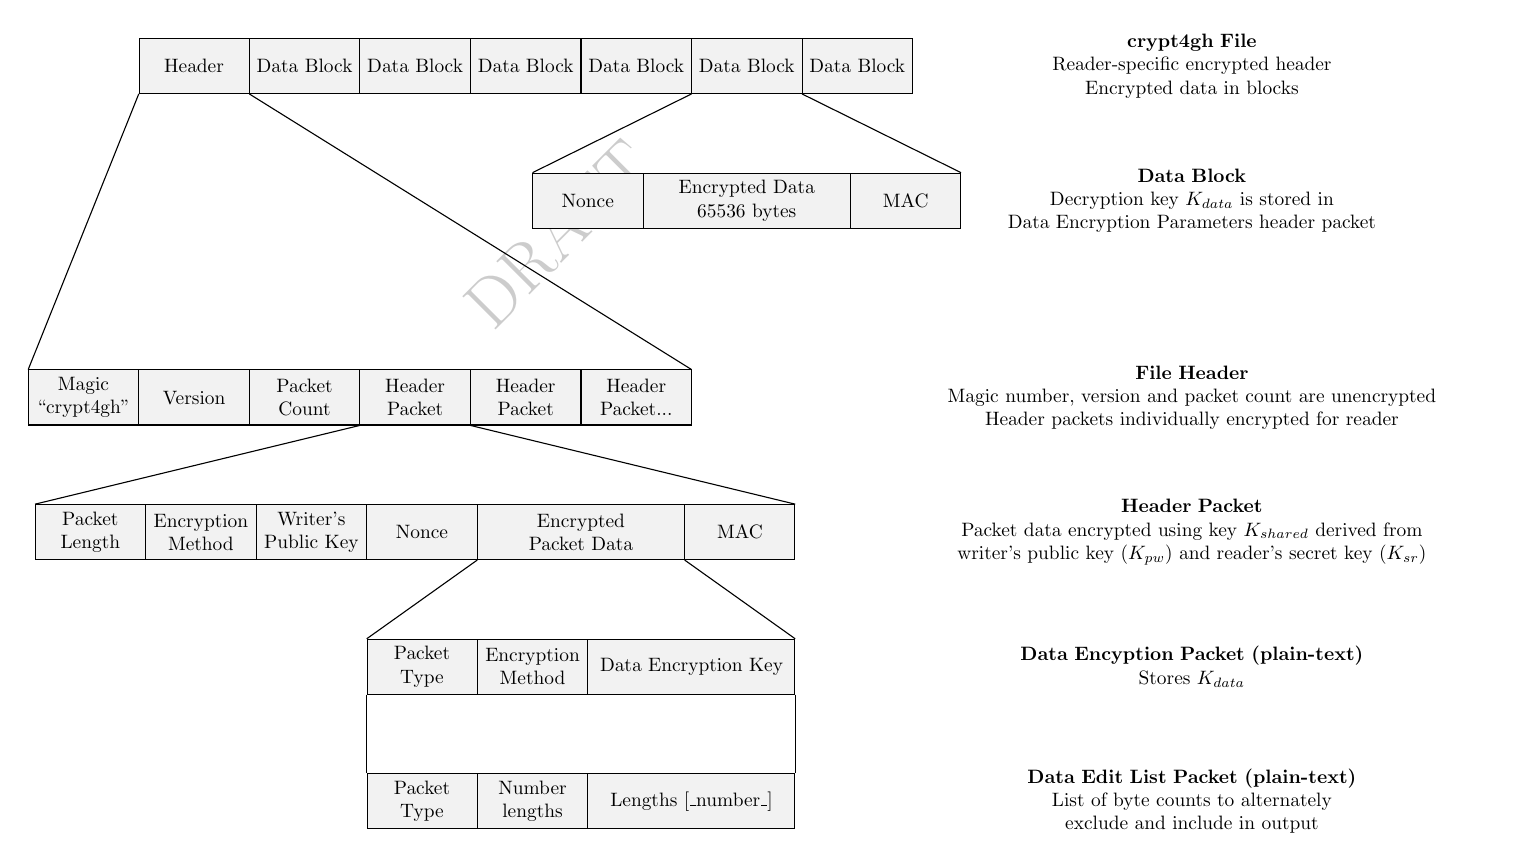
\begin{tikzpicture}[
    every node/.style={scale=0.7},
    boxes/.style={rectangle split,rectangle split parts=#1,draw,rectangle split horizontal,text width=5em,align=center,minimum height=1cm,fill=black!5,on grid},
    notes/.style={text width=20em,align=center,minimum height=1cm,on grid},
  ]
\node (file) [boxes=7] {
\nodepart{one}Header
\nodepart{two}Data Block
\nodepart{three}Data Block
\nodepart{four}Data Block
\nodepart{five}Data Block
\nodepart{six}Data Block
\nodepart{seven}Data Block
};
\node (file notes) [notes,right=of file.east] {
  \textbf{crypt4gh File} \\
  Reader-specific encrypted header \\
  Encrypted data in blocks
};

\node (data block) [boxes=3,below=1 of file.six south] {
\nodepart{one}Nonce
\nodepart[text width=10em]{two}Encrypted Data \\ 65536 bytes
\nodepart{three}MAC
};
\draw (file.five split south) to (data block.north west);
\draw (file.six split south) to (data block.north east);
\node (data block notes) at (data block -| file notes) [notes] {
  \textbf{Data Block} \\
  Decryption key $K_{data}$ is stored in \\
  Data Encryption Parameters header packet
};

\node (header) [boxes=6,below=3.5 of file.two split south] {
\nodepart{one}Magic \\ ``crypt4gh''
\nodepart{two}Version
\nodepart{three}Packet Count
\nodepart{four}Header Packet
\nodepart{five}Header Packet
\nodepart{six}Header Packet...
};
\draw (file.south west) to (header.north west);
\draw (file.one split south) to (header.north east);
\node (header notes) at (header -| file notes) [notes,text width=30em] {
  \textbf{File Header} \\
  Magic number, version and packet count are unencrypted \\
  Header packets individually encrypted for reader
};

\node (header packet) [boxes=6,below=of header.four south] {
\nodepart{one}Packet Length
\nodepart{two}Encryption Method
\nodepart{three}Writer's Public Key
\nodepart{four}Nonce
\nodepart[text width=10em]{five}Encrypted Packet Data
\nodepart{six}MAC
};
\draw (header.three split south) to (header packet.north west);
\draw (header.four split south) to (header packet.north east);
\node (header packet notes) at (header packet -| file notes) [notes,text width=30em] {
  \textbf{Header Packet} \\
  Packet data encrypted using key $K_{shared}$ derived from writer's public key ($K_{pw}$) and reader's secret key ($K_{sr}$)
};

\node (data encryption packet) [boxes=3,below=of header packet.five south] {
\nodepart{one}Packet Type
\nodepart{two}Encryption Method
\nodepart[text width=10em]{three}Data Encryption Key
};
\draw (header packet.four split south) to (data encryption packet.north west);
\draw (header packet.five split south) to (data encryption packet.north east);
\node (data encryption packet notes) at (data encryption packet -| file notes) [notes] {
  \textbf{Data Encyption Packet (plain-text)} \\
  Stores $K_{data}$
};

\node (data edit list) [boxes=3,below=of data encryption packet.south] {
\nodepart{one}Packet Type
\nodepart{two}Number lengths
\nodepart[text width=10em]{three}Lengths [\_number\_]
};
\draw (data encryption packet.south west) to (data edit list.north west);
\draw (data encryption packet.south east) to (data edit list.north east);
\node (data edit list notes) at (data edit list -| file notes) [notes] {
  \textbf{Data Edit List Packet (plain-text)} \\
  List of byte counts to alternately exclude and include in output
};
\end{tikzpicture}
\end{center}

The encrypted file structure, shown in the diagram above, consists of the following parts:

\begin{itemize}
\item A header containing: a ``magic'' string, version number and header packet count.
\begin{itemize}
\item A ``magic'' string for file type identification.
\item A version number.
\item The header packet count.
\item One or more header packets containing:
\begin{itemize}
\item The packet length in bytes.
\item The method used to encrypt the header packet data.
\item The writer's public key  ($K_{pw}$) used to encrypt the header packet data.
This is needed (along with the reader's secret key $K_{sr}$)
to calculate the shared key used to encrypt the header packet.
\item A random ``nonce'', also required for decryption.
\item The encrypted data for the header packet.
\item A MAC calculated over the encrypted header packet data.
\end{itemize}
The first item in the encrypted header packet data is a code indicating the packet type.
This is followed by type-specific data, described in section~\ref{overview:header_packet_types}.
\end{itemize}
\item The encrypted data.
This is the actual application data, stored in a sequence of blocks containing:
\begin{itemize}
\item A random ``nonce'', needed for decryption.
\item 64 kilobytes of encrypted data (the last block may contain less than this).
\item A MAC calculated over the encrypted data.
\end{itemize}
\end{itemize}

\subsection{Header Packet Types}\label{overview:header_packet_types}
There are two types of header packet:
\begin{itemize}
\item Data encryption key packets.

These describe the parameters used to encrypt one or more of the data blocks.
They contain a code indicating the type of encryption, and the symmetric key ($K_{data}$) needed to decrypt the data.

If parts of the data have been encrypted with different keys, more than one of this packet type will be present.

\item Data edit list packets.

These packets allow parts of the data to be discarded after decryption.
They can be used to avoid having to decrypt and re-encrypt files during splicing operations.

For example, a user may want to extract the blocks corresponding to Chromosome X from a CRAM file and store them
in a new file.
If the start and end points of the extract do not correspond to a 64Kbyte data block boundary, they would normally
have to decrypt all of the data blocks covering the region, discard a few bytes from the start and end, re-encrypt the
remaining data and store it in a new file.

The data edit list enables a simpler solution where the necessary encrypted data blocks are copied directly into
the new file.
On reading, the data blocks are decrypted and then the edit list is used to find out which parts of the unencrypted
data should be discarded.
\end{itemize}

\subsection{Encoding For Multiple Public/Secret Key Pairs}

It is sometimes useful to encrypt files so that they can be accessed using more than one secret key ($K_{sr}$).
For example, multiple members of a team may need to access to a file with their own key.

To allow this,
the header packet data is encrypted using each reader's public key ($K_{pr}$) and stored in a separate header packet
for each individual reader.

Where this is done, it is likely that anyone reading the file will only have the correct secret key ($K_{sr}$) for a
subset of the header packets.
Attempting to decode a header packet with the wrong key will result in a failure to verify the MAC stored in the file.
When this happens, implementations should ignore the undecodable header packet and move on to the next one.
Failing to decrypt a packet in this way SHOULD NOT cause an error to be reported;
however an error MUST be raised if, on reaching the end of the header,
it has not been possible to decrypt at least one data encryption key packet.

\section{Detailed Specification}
\subsection{Overall Conventions}
\subsubsection{Hexadecimal Numbers}
Hexadecimal values are written using the digits 0-9, and letters a-f for values 10-15.
Values are written with the most-significant digit on the left, and prefixed with "0x".

\subsubsection{Byte Ordering}
The basic data size is the byte (8 bits).
All multi-byte values are stored in least-significant byte first (``little-endian'') order.
For example, the value 1234 decimal (0x4d2) is stored as the byte stream 0xd2 0x04.

\subsubsection{Integer Types}
Integers can be either signed or unsigned.
Signed values are stored in two's complement form.

\subsubsection{Multi-byte Integer Types}
\begin{center}
\begin{tabular}{l l l l}
\hline
\textbf{Name} & \textbf{Byte Ordering} & \textbf{Integer Type} & \textbf{Size (bytes)} \\
\hline
byte & & unsigned & 1 \\
le\_int32 & little-endian & signed & 4 \\
le\_uint32 & little-endian & unsigned & 4 \\
le\_int64 & little-endian & signed & 8 \\
le\_uint64 & little-endian & unsigned & 8 \\
le\_uint96 & little-endian & unsigned & 12 \\
\end{tabular}
\end{center}

\subsubsection{Structures}
Structure types may be defined (in C-like notation) for convenience.

\begin{verbatim}
struct demo {
  byte string[8];
  le_int32 number1;
  le_uint64 number2;
};
\end{verbatim}

When structures are serialised to a file, elements are written in the given order with no padding between them.
The above structure would be written as twenty bytes - eight for the array `string', four for the integer `number1',
and eight for the integer `number2'.

\subsubsection{Enumerated Types}
Enumerated types may only take one of a given set of values.
The data type used to store the enumerated value is given in angle brackets after the type name.
Every element of an enumerated type must be assigned a value.
It is not valid to compare values between two enumerated types,
except to compare for (in)equality.

\begin{verbatim}
enum Animal<le_uint32> {
  cat    = 1;
  dog    = 2;
  rabbit = 3;
};
\end{verbatim}

\subsubsection{Variants}
Parts of structures may vary depending on information available at the time of decoding.
Which variant to use is selected by an enumerated type.
There must be a case for every possible enumerated value.
Cases have limited fall-through.
Consecutive cases with no fields in between all contain the same fields.

\begin{verbatim}
struct AnimalFeatures {
  select (enum Animal) {
    case cat:
    case dog:
      le_uint32 hairyness;
      le_uint32 whisker_length;

    case rabbit:
      le_uint32 ear_length;
  };
};
\end{verbatim}

For the `cat' and `dog' cases, `struct AnimalFeatures' is eight bytes long and contains two unsigned four-byte
little-endian values.
For the `rabbit' case it is four bytes long and contains a single four-byte little-endian value.

If the cases are different lengths (as above), then the size of the overall structure depends on the variant chosen.
There is NO padding to make the cases the same length unless it is explicitly defined.

\subsection{Header}

The file starts with a header, with the following structure:

\begin{verbatim}
struct Header {
  byte                          magic_number[8];
  le_uint32                     version;
  le_uint32                     header_packet_count;
  Encrypted_header_packet       header_packets[header_packet_count]
};
\end{verbatim}

The \kw{magic\_number} is the ASCII representation of the string ``crypt4gh''.

The version number is stored as a four-byte little-endian unsigned integer.
The current version number is 1.

The current byte representation of the magic number and version is:
\begin{verbatim}
0x63 0x72 0x79 0x70 0x74 0x34 0x67 0x68 0x01 0x00 0x00 0x00
============= magic_number============= ===== version =====
\end{verbatim}

\kw{header\_packet\_count} is the number of header packets that follow.

\subsubsection{Header Packets}\label{header:encryption}

The header packets are defined as:

\begin{verbatim}
enum Header_encryption_method<le_uint32> {
  X25519_chacha20_ietf_poly1305 = 0;
};

struct Header_packet {
  le_uint32                           packet_length;
  Header_encryption_method<le_uint32> packet_encryption;

  select (packet_encryption) {
    case X25519_chacha20_ietf_poly1305:
      byte   writer_public_key[32];
      byte   nonce[12];
  };

  byte encrypted_payload[];

  select (packet_encryption) {
    case X25519_chacha20_ietf_poly1305:
      byte MAC[16];
  };
};
\end{verbatim}

\kw{packet\_length} is the length of the entire header packet (including the \kw{packet\_length} itself).
To prevent packet types from being guessed by looking at the size, it is permitted for the \kw{packet\_length} to be
longer than strictly needed to encode all of the packet data.
Any remaining space after the actual data should be padded in a suitable manner (for example by setting it to zero)
and encrypted.

\kw{packet\_encryption} is the encryption method used for this header packet.

\kw{writer\_public\_key} ($K_{pw}$) and \kw{nonce} are parameters needed to decrypt the \kw{encrypted\_payload} in the
packet.

\kw{encrypted\_payload} is the encrypted part of the header packet, for which the plain-text is described below.

\kw{MAC} is a message authentication code calculated over the encrypted data.

Implementations should ignore any header packets that they cannot decrypt successfully, as these may have
been intended for a different reader.

\subsubsection{Header packet encrypted payload}

The \kw{encrypted\_payload} part of the header packet contains the following plain-text:

\begin{verbatim}
enum Header_packet_type<le_uint32> {
  data_encryption_parameters = 0;
  data_edit_list = 1;
};

enum Data_encryption_method<le_uint32> {
  chacha20_ietf_poly1305 = 0;
};

struct Encrypted_header_packet {
  Header_packet_type<le_uint32> packet_type;

  select (packet_type) {
    case data_encryption_parameters:
      enum Data_encryption_method<le_uint32>  data_encryption_method;
      select (data_encryption_method) {
        case chacha20_ietf_poly1305:
          byte  data_key[32];
      };

    case data_edit_list:
      le_uint32 number_lengths;
      le_uint64 lengths[number_lengths];
  };
};
\end{verbatim}

\kw{packet\_type} defines what sort of data packet this is.

\subsubsection{data\_encryption\_parameters packet}\label{header:data_encryption_parameters}

This packet contains the parameters needed to decrypt the data part of the file.

\kw{data\_encryption\_method} is an enumerated type that describes the type of encryption used.

\kw{data\_key} is the symmetric key $K_{data}$ used to decode the data section.

To allow parts of the data to be encrypted with different $K_{data}$ keys,
more than one of this packet type may be present.
If there is more than one, the \kw{data\_encryption\_method} MUST be the same for all of them to prevent problems
with random access in the encrypted file.

\subsubsection{data\_edit\_list packet}

This packet contains a list of edits that should be applied to the plain-text data following decryption.

\kw{number\_lengths} is the number of items in the \kw{lengths} array.

\kw{lengths} is an array of byte counts.

Application of the edit list to the plain-text is described in section~\ref{data:edit_list}.

It is not permitted to have more than one edit list.
If more than one edit list is present, the file SHOULD be rejected.

\subsection{Header packet encryption}

\subsubsection{X25519\_chacha20\_ietf\_poly1305 Encryption}~\label{header:X25519}

This method uses Elliptic Curve Diffie-Hellman key exchange with additional hashing to generate a shared
key ($K_{shared}$).
$K_{shared}$ is then used along with a randomly-generated nonce to encrypt the header packet data using the
ChaCha20-IETF-Poly1305 construction.
The elliptic curve algorithm used is X25519, described in section 5 of \cite{RFC7748}.

Encryption requires the writer's public and secret keys ($K_{pw}$ and $K_{sw}$), the reader's public key ($K_{pr}$)
and a nonce ($N$).

The nonce is a unique initialisation vector.
In ChaCha20-IETF-Poly1305 it is 12 bytes long.
This value MUST be unique for each packet encrypted with the same reader's and writer's keys.
The best way to ensure this is to generate a value with a cryptographically-secure random number generator.

The secret keys MUST be generated using a cryptographically-secure random number generator.
The corresponding public keys are derived using the method in section 6.1 of \cite{RFC7748}.

$K_p = X25519(K_s, 9)$

The writer's secret key and the reader's public key are used to generate a Diffie-Hellman shared key as described in
section 6.1 of \cite{RFC7748}.

$K_{dh} = X25519(K_{sw}, K_{pr})$

As the X25519 algorithm does not produce a completely uniform bit distribution,
and many possible $(K_{sw}, K_{pr})$ pairs can produce the same output,
the Diffie-Hellman key is hashed along with the two public keys to produce the final shared key.
The hash function used to do this is Blake2b, as described in \cite{RFC7693}.

$K_{shared} = Blake2b(K_{dh} || K_{pr} || K_{pw})$

As ChaCha20 uses a 32-byte key, only the first 32 bytes of $K_{shared}$ are used; the rest are discarded.

The header packet type, data and any padding is then encrypted using the method described in the
chacha20\_ietf\_poly1305 Encryption section~\ref{data:chacha20_encryption}.
Note that header packets are not segmented; they are always encrypted in a single block.

Finally, the packet length, encryption type, writer's public key $K_{pw}$,
the nonce $N$ and the encrypted header packet data are combined to make the header packet.

For extra security, writers MAY choose to discard the writer's secret key $K_{sw}$ after use.
Due to the symmetry of the Diffie-Hellman algorithm, the holder of either secret key can regenerate the shared
key as long as the other public key is known.
Deleting the writer's key $K_{sw}$ ensures only the holder of the reader's secret key $K_{sr}$ can decode the header
packet.
As long as the writer uses randomly-generated keys, it also makes accidental nonce reuse very unlikely.

\subsubsection{X25519\_chacha20\_ietf\_poly1305 Decryption}

To decrypt the header packet, the reader obtains the writer's public key $K_{pw}$ and the nonce from the beginning
of the packet.
Also needed are the reader's public and secret keys ($K_{pr}$ and $K_{sr}$).

The Diffie-Helman key is obtained using:

$K_{dh} = X25519(K_{sr}, K_{pw})$

This is then hashed to obtain the shared key (again only the first 32 bytes are retained):

$K_{shared} = Blake2b(K_{dh} || K_{pr} || K_{pw})$

The resulting key $K_{shared}$ and nonce $N$ are then used to decrypt the remainder of the packet.

If the header packet was intended for a different reader, the reader will be unable to decode the header packet
as the Poly1305 MAC will be incorrect.
This should not be considered an error.

\subsubsection{Reading the header}

The reader should check that the \kw{magic\_number} and \kw{version} in the header match the expected values.

It should then attempt to decode all of the header packets, ignoring any that do not decrypt successfully
(detected by a failure to verify the MAC).
At the end of this process the reader should have decoded at least one \kw{data\_encryption\_parameters} packet.
If no such packet was decoded, it SHOULD report an error.
If more than one is present, they should all have the same \kw{data\_encryption\_method}, otherwise the reader
SHOULD report an error.
The reader should store all of the keys that it has decoded in a list for use when decoding the encrypted data section.

If a \kw{data\_edit\_list} packet is found, the reader should store it for use while processing the data blocks.
If more than one \kw{data\_edit\_list} packet is present, the file SHOULD be rejected.

\subsection{Encrypted Data}\label{data:encryption}
\subsubsection{chacha20\_ietf\_poly1305 Encryption}\label{data:chacha20_encryption}

ChaCha20 is a stream cipher which maps a 256-bit key, nonce and counter to a 512-bit key-stream block.
In IETF mode the nonce is 96 bits long and the counter is 32 bits.
The counter starts at 1, and is incremented by 1 for each successive key-stream block.
The cipher-text is the plain-text message combined with the key-stream using the bit-wise exclusive-or operation.

Poly1305 is used to generate a 16-byte message authentication code (MAC) over the cipher-text.
As the MAC is generated over the entire cipher-text it is not possible to authenticate partially decrypted data.

ChaCha20 and Poly1305 are combined using the AEAD construction described in section 2.8 of \cite{RFC8439}.
This construction allows additional authenticated data (AAD) to be included in the Poly1305 MAC calculation.
For the purposes of this format, the AAD is zero bytes long.

\subsubsection{Segmenting the input}

To allow random access without having to authenticate the entire file, the plain-text is divided into 65536-byte
(64KiB) segments.
If the plain-text is not a multiple of 64KiB long, the last segment will be shorter.
Each segment is encrypted using the method defined in the header.
The nonce used to encrypt the segment is then stored, followed by the encrypted data, and then the MAC.

\begin{verbatim}
struct Segment {
  select (method) {
    case chacha20_ietf_poly1305:
      byte    nonce[12];
      byte[]  encrypted_data;
      byte    mac[16];
  };
};
\end{verbatim}

The addition of the \kw{nonce} and \kw{mac} bytes will expand the data slightly.
For chacha20\_ietf\_poly1305, this expansion will be 28 bytes, so a 65536 byte plain-text input will become a 65564
byte encrypted and authenticated cipher-text output.

\section{Decryption}

\subsection{chacha20\_ietf\_poly1305 Decryption}

The cipher-text is decrypted by authenticating and decrypting the segment(s) enclosing the requested byte range $[P;Q]$,
where $P<Q$.
For a range starting at position $P$, the location of the segment \kw{seg\_start} containing that position must
first be found.
For the chacha20\_ietf\_poly1305 method, when no edit list is in use, this can be done using the formula:

\begin{verbatim}
seg_start = header_len + floor(P/65536) * 65564
\end{verbatim}

For an encrypted segment starting at position \kw{seg\_start}, the nonce, then the 65536 bytes of cipher-text
(possibly fewer of it was the last segment), and finally the MAC are read.

An authentication tag is calculated over the cipher-text from that segment, and bit-wise compared to the MAC.
The cipher-text is authenticated if and only if the tags match.
If more than one key ($K_{data}$) was included in the header,
each should be tried in turn until either one authenticates correctly or no keys are left to try.
An error MUST be reported if the cipher-text is not authenticated.

The key $K_{data}$ and nonce $N$ are then used to decrypt the cipher-text for the segment, returning the plain-text.
Successive segments are decrypted, until the segment containing position $Q$ is reached.
The plain-text segments are concatenated to form the resulting output, discarding $P \mathbin{\%} 65536$ bytes from
the beginning of the first segment and retaining $Q \mathbin{\%} 65536$ bytes of the last one.

If more than one key ($K_{data}$) is in use,
readers can speed up decryption by trying the previous successful key first when attempting to authenticate each block.
However, this does open up a possible timing attack where an observer watching the decoding process can find
out where key changes occur due to the extra time needed to select the new key at these points.
If this is unacceptable, readers could either try each key for every block (although this may still be vulnerable
to timing attacks which try to detect which key was successful); or simply insist that only one key is used for
the whole file.

\subsection{Edit List}\label{data:edit_list}

The edit list is designed to assist splicing of encrypted files (for example to remove parts that are not needed
for later analysis) without having to decrypt and re-encrypt the entire file.
It is only possible to splice crypt4gh files at the 64K encryption block boundaries.
The edit list can be used to work around this limitation by describing which parts of the unencrypted blocks
should be discarded to give the final desired plain-text.

The following algorithm describes how to apply the edit list $edlist$ to unencrypted text $input$ to return
the desired edited plain-text.
In this algorithm, function \textsc{IsEmpty} returns true if a list is empty and false if not.
Function \textsc{RemoveFirst} removes the first item from a list and returns it.
\textsc{length} returns the length of a string.
\textsc{substr} returns part of a string from a given zero-based position and with a given length (or shorter if the
requested part extends beyond the end of the input string).
\textsc{StringConcatenate} returns the string concatenation of its input parameters in order from left to right.

\begin{algorithmic}[1]
\Function{ApplyEditList}{$edlist,\ input$}
\If{\Call{IsEmpty}{edlist}}
  \State \textbf{return} $input$\Comment{Trivial case with no edit list}
\EndIf
\settowidth{\maxwidth}{output}
\State \algalign{output}{\gets} ``''\Comment{Initial output is empty}
\State \algalign{pos}{\gets} $0$\Comment{Current position in the unedited plain-text}
\State \algalign{len}{\gets} \Call{length}{input}\Comment{Length of input string}
\Repeat
  \settowidth{\maxwidth}{discard}
  \State \algalign{discard}{\gets} \Call{RemoveFirst}{edlist}\Comment{Pull number of bytes to discard from list}
  \State \algalign{pos}{\gets} $pos + discard$
  \If{\Call{IsEmpty}{edlist}}
     \settowidth{\maxwidth}{output}
     \State \algalign{part}{\gets} \Call{substr}{$input, pos, len - pos$}\Comment{Append the remainder of $input$}
     \State \algalign{output}{\gets} \Call{StringConcatenate}{$output,\ part$}
  \Else
     \settowidth{\maxwidth}{output}
     \State \algalign{keep}{\gets} \Call{RemoveFirst}{edlist}\Comment{Pull number of bytes to keep from the list}
     \State \algalign{part}{\gets} \Call{substr}{$input, pos, keep$}\Comment{Append this part to $output$}
     \State \algalign{output}{\gets} \Call{StringConcatenate}{$output,\ part$}
     \State \algalign{pos}{\gets} $pos + keep$
  \EndIf
\Until{\Call{IsEmpty}{edlist}}
\State \textbf{return} $output$
\EndFunction
\end{algorithmic}

\subsubsection{Example}

Imagine that for some reason we have made an encrypted copy of ERR2436651.
\footnote{The data for this example comes from \url{ftp://ftp.sra.ebi.ac.uk/vol1/run/ERR243/ERR2436651/}.}

We would like to make a new encrypted file including just the data aligned to ChrII,
without having to decrypt and re-encrypt the desired data.
The new file will need to include the following items (note that byte ranges are zero-based inclusive):

\begin{enumerate}
\item A crypt4gh header containing the keys needed to decrypt the file.
\item The CRAM header (plain-text bytes 0 to 7852).
\item ChrII data (plain-text bytes 145110 to 453038).
\item The CRAM end-of-file block (plain-text bytes 5485074 to last byte of file at 5485111).
\end{enumerate}

None of these byte ranges align with 64K boundaries.
To avoid the need to decrypt and re-encrypt the data,
an edit list can be added to the crypt4gh header and the byte ranges are expanded to complete encrypted blocks.
After this the list of items to send will be:

\begin{enumerate}
\item A crypt4gh header containing the keys needed to decrypt the file and an edit list.
\item The CRAM header (plain-text bytes 0 to 65535).
\item ChrII data (plain-text bytes 131072 to 458751).
\item The CRAM end-of-file block (plain-text bytes 5439488 to last byte of file at 5485111).
\end{enumerate}

These segments will be concatenated to make the new file,
so in this case to obtain the desired data the edit list will contain the values:
\begin{center}
$[0, 7853, 71721, 307929, 51299, 38]$
\end{center}

Which means:

\begin{itemize}
\item Discard zero bytes from the start.
\item Keep 7853 bytes (the CRAM header).
\item Discard 57683 bytes (following the CRAM header) + 14038 bytes (before ChrII data) = 71721 bytes in total.
\item Keep 307929 bytes (ChrII data).
\item Discard 5713 bytes (following ChrII) + 45586 bytes (before the EOF block) = 51299 bytes in total.
\item Keep 38 bytes (EOF block).
This could actually be left out as it extends all the way to the end of the file.
\end{itemize}

\section{Security Considerations}
\subsection{Threat Analysis}
This format is primarily designed to protect files at rest and in transport from accidental disclosure.
Attackers are assumed to have read access to encrypted files.
Even if this is the case,
it should not be possible to decrypt the file without access to the reader's secret key ($K_{sr}$).

Some file formats use supplementary files, for example external indices.
In some cases it may be possible to deduce information about the data file from the supplementary one.
For example, it is usually trivial to determine gender from a BAM index,
and it may also be possible to detect certain other genetic conditions.
Where the main data file needs to be encrypted, such supplementary files MUST be encrypted as well.

While key management is out of scope for this document,
it should be noted that it is important that attackers are not able to access secret keys.
Implementations MUST ensure that secret keys are kept in a secure manner.

Attackers with write access to files will not be able to make changes to individual blocks as
(without access to the decryption key) they will not be able to calculate the correct MAC on the new version.
Such an attacker can, however, make block-level changes such as removing or reordering blocks.
An attacker with access to the reader's public key ($K_{pr}$) will also be able to add entire blocks by inserting a new
data\_encryption\_parameters packet in the header, and using the key stored in it to encrypt the new block.

It is expected that files using this format will be decrypted in memory for processing.
There is a risk of data being leaked either directly or through a side-channel (many of which are difficult to defend
against).
It is very likely that attackers who gain access to machines analysing data in encrypted files will be able
to make deductions about the file contents, or in the worst case either extract the entire decrypted file or
obtain the decryption keys.

Implementations SHOULD use cryptographic libraries hardened against common side-channel (e.g. timing) attacks.
Implementations MUST keep secret material as safe as possible.
For example, keys should ideally be locked into memory to avoid them being paged to a swap file.
Keys should also be securely erased as soon as they are no longer needed.
Any intermediate files written out during processing SHOULD be encrypted.

Deployments MUST take precautions to prevent attackers from accessing data while it is processed.
Note that the following list is not exhaustive.
\begin{itemize}
\item Software MUST be kept up to date for security patches.
\item Data should not be processed on machines shared by more than one user.
\item Local file systems and swap partitions should be encrypted.
\item Debugging interfaces (for example ptrace) should be disabled.
\item Machines should not be running any unnecessary processes or services.
\item Firewall rules should be used to restrict network access to only sites needed for processing the data.
\item Users should avoid running processes like web browsers that can run arbitrary code downloaded from the Internet
(even if the code is run in a sand-box environment) on a machine where encrypted data is being processed.
\end{itemize}

\subsection{Selection of Keys}
The security of the format depends on attackers not being able to guess secret keys ($K_{sr}$ and $K_{sw}$)
or the data encryption key ($K_{data}$).
The keys MUST be generated using a cryptographically-secure pseudo-random number generator.
This makes the chance of guessing a key vanishingly small.

\subsection{Nonce selection}
All header packets encrypted with the same combination of writer's secret key ($K_{sw}$)
and reader's public key ($K_{pr}$) MUST use a unique nonce.
If the writer uses the same secret key ($K_{sw}$) for more than one file then all nonces MUST be unique across all
files made with that key.
As each file will only include a few header packets this restriction can be fulfilled by generating each nonce
using a cryptographically-secure random number generator.
If the writer uses a randomly-generated $K_{sw}$ for each file, or even each header packet, the risk of nonce reuse in
the header is almost completely eliminated.

All data segments encrypted with the same key MUST use a unique nonce.
One way to ensure this is to choose a random starting point and then use a counter or linear-feedback shift
register to generate the nonce for each segment.
This method guarantees a unique value even for very long files.

For a 96-bit nonce, it may be acceptable to generate each one using a cryptographically-secure pseudo-random number
generator.
Care should be taken to ensure that the random number generator is capable of generating a long enough stream
of unique values.
Due to the birthday problem, this method will have a non-zero (but very small) probability of failing.
For example, a file of 24 Terabytes will have a reused nonce with probability of approximately $10^{-12}$

\subsection{Message Forgery}
Using ChaCha20-IETF-Poly1305 authenticates the content of each header packet and each segment of the encrypted
cipher-text.
It does not protect against the addition or removal of header packets, or the addition, removal or rearrangement
of data segments.
crypt4gh files are not signed, so there is no direct way to prove that a file was created by a given writer.

\subsection{No File Updates Permitted}
Implementations MUST NOT update encrypted files.
Once written, a section of the file must never be altered.

\bibliographystyle{abstract}

\begin{thebibliography}{XXXXXXX}

% Normative references
\subsection{Normative References}

\bibitem[RFC2119]{RFC2119}
  Bradner, S.,\\
  \emph{"Key words for use in RFCs to Indicate Requirement Levels", BCP 14, RFC 2119},\\
  \url{https://www.rfc-editor.org/info/rfc2119},\\
  March 1997

\bibitem[RFC7693]{RFC7693}
  Saarinen, M.J., Aumasson, J.P.\\
  \emph{"The BLAKE2 Cryptographic Hash and Message Authentication Code (MAC)", RFC7693},\\
  \url{https://tools.ietf.org/html/rfc7693},\\
  November 2015

\bibitem[RFC7748]{RFC7748}
  A. Langley, Google, M. Hamburg, Rambus Cryptography Research, S. Turner, sn3rd,\\
  \emph{"Elliptic Curves for Security", RFC7748},\\
  \url{https://tools.ietf.org/html/rfc7748},\\
  January 2016

\bibitem[RFC8032]{RFC8032}
  S. Josefsson, SJD AB, I. Liusvaara,\\
  \emph{"Edwards-Curve Digital Signature Algorithm (EdDSA)", RFC8032},\\
  \url{https://tools.ietf.org/html/rfc8032},\\
  January 2017

\bibitem[RFC8439]{RFC8439}
  Y. Nir, Dell EMC, A. Langley, Google, Inc.,\\
  \emph{"ChaCha20 and Poly1305 for IETF Protocols", RFC8439},\\
  \url{https://tools.ietf.org/html/rfc8439},\\
  June 2018

% Informational references
\subsection{Informational References}

\bibitem[RFC4880]{RFC4880}
  Callas, J., PGP Corporation, Donnerhacke, L., IKS GmbH, Finney, H., PGP Corporation, Shaw, D., Thayer, R.,\\
  \emph{"OpenPGP Message Format", RFC 4880},\\
  \url{https://www.rfc-editor.org/info/rfc4880},\\
  November 2007.

\bibitem[RFC8446]{RFC8446}
  Rescorla, E.,\\
  \emph{"The Transport Layer Security (TLS) Protocol Version 1.3", RFC 8446},\\
  \url{https://www.rfc-editor.org/info/rfc8446},\\
  August 2018.

\bibitem[RFC8551]{RFC8551}
  Schaad, J., August Cellars, Ramsdell, B., Brute Squad Labs, Inc., Turner, S.,\\
  \emph{"Secure/Multipurpose Internet Mail Extensions (S/MIME) Version 4.0 Message Specification", RFC 8551},\\
  \url{https://www.rfc-editor.org/info/rfc8551},\\
  April 2019.

\bibitem[AE LIMITS]{AE LIMITS}
  Luykx, A., Paterson, K.,\\
  \emph{"Limits on Authenticated Encryption Use in TLS"},\\
  \url{http://www.isg.rhul.ac.uk/~kp/TLS-AEbounds.pdf},
  August 2017.

\bibitem[Curve25519]{Curve25519}
  Bernstein, Daniel J.,\\
  \emph{"Curve25519: New Diffie-Hellman Speed Records"},\\
  \url{https://doi.org/10.1007%2F11745853_14},\\
  2006.

\bibitem[SafeCurves]{SafeCurves}
  Bernstein, Daniel J., Lange, Tanja,\\
  \emph{"SafeCurves: choosing safe curves for elliptic-curve cryptography."},\\
  \url{https://safecurves.cr.yp.to},\\
  accessed 22 July 2019.

\bibitem[Blake2]{Blake2}
  Aumasson, J-P., Neves, S., Wilcox-O’Hearn, Z., Winnerlein, C.,\\
  \emph{"BLAKE2: simpler, smaller, fast as MD5"},\\
  \url{https://eprint.iacr.org/2013/322.pdf},\\
  2013.

\bibitem[Post-Quantum]{Post-Quantum}
  Alagic, G., Alperin-Sheriff, J., Apon, D., Cooper, D., Dang, Q., Miller, C., Moody, D., Peralta, R., Perlner, R., Robinson, A., Smith-Tone, D, Liu, Y-K.,\\
  \emph{"Status Report on the First Round of the NIST Post-Quantum Cryptography Standardization Process"},\\
  \url{https://doi.org/10.6028/NIST.IR.8240},\\
  January 2019.

\bibitem[htsget]{htsget}
  Kelleher, J., Lin, M., Albach, C. H., Birney, E., Davies, R., Gourtovaia, M., Glazer, D., Gonzalez, C. Y., Jackson, D. K., Kemp, A., Marshall, J., Nowak, A., Senf, A., Tovar-Corona, J. M., Vikhorev, A., Keane, T. M., GA4GH Streaming Task Team
  \emph{"htsget: a protocol for securely streaming genomic data"}
  \url{https://doi.org/10.1093/bioinformatics/bty492}
  June 2018.

\end{thebibliography}

\appendix
\section{Rationale}

Using authenticated encryption in individual segments mirrors solutions like Transport Layer
Security (TLS) as described in~\cite{RFC8446} and prevents undetected modification of segments.
Dividing the file into fixed-size (except at the end) blocks allows random-access into the encrypted file.
The format is also designed to allow streaming reads and writes;
in particular when writing no more than 64 Kbytes of plain-text needs to be known at any point.

While the standard allows for multiple encryption methods, only one choice is currently allowed.
This simplifies implementations while allowing the current choice to be replaced in a future revision if it is found
to have any vulnerabilities.
The criteria for choosing encryption methods included having strong security guarantees, good library support
and being used in other common standards like TLS version 1.3.

\subsection{Symmetric Encryption}

For symmetric encryption, the main candidates for authenticated encryption were AES-GCM and ChaCha20-Poly1305.
Both have good security guarantees, and thanks to their use in TLS 1.3 both have good library support.
ChaCha20-Poly1305 was chosen because it allows much longer files to be encrypted.
See~\cite{AE LIMITS} for a comparison although note that our ``messages'' are $2^{16}$ bytes long,
while the figures in the paper are for $2^{14}$ bytes.

There are three common ChaCha20-Poly1305 constructions original, ChaCha20-IETF-Poly1305, and XChaCha20-Poly1305.
The main differences are the length of the nonce and the maximum message size allowed using a single nonce.
ChaCha20-IETF-Poly1305 was chosen because it has the best library support thanks to its use in Internet Engineering
Task Force protocols and the nonce length allows a very large number of messages to be encrypted under a single key.
The message length restriction of ChaCha20-IETF-Poly1305 ($64*2^{32}-64$ bytes) is not a problem as our ``messages''
are at most 64 Kbytes long.

\subsection{Public-key Algorithm}

For public-key encryption Elliptic Curve Diffie-Hellman using X25519 was chosen.
Elliptic Curve Diffie-Hellman is faster and uses smaller keys than methods such as RSA or traditional Diffie–Hellman.
X25519 is based on Curve25519 which allows fast implementations, has good security properties~\cite{Curve25519}
and has been constructed to avoid a number of possible implementation problems~\cite{SafeCurves}.
X25519 is used in TLS version 1.3, S/MIME 4.0~\cite{RFC8551} and many other protocols, and has good library support.

X25519 is used to generate a shared key.
While this key could be used on its own, its properties are not ideal because many secret/public key pairs can
generate the same key and the bit distribution across the key is not completely uniform.
To enhance the key, it is concatenated with the two public keys used in the key exchange and then passed through
a secure hash function.
The chosen hash function (Blake2b) has good library support,
is faster than SHA-2 and has similar security to that of SHA-3~\cite{Blake2}.

The generated shared key $K_{shared}$ is used as the secret material for symmetric encryption of the header packet data.
As it is already used for encrypting the data blocks, the method chosen for this is ChaCha20-IETF-Poly1305.

Like other ECDH schemes, X25519 is not resistant to attack using a quantum computer.
At the time of writing, quantum-computing resistant algorithms are undergoing standardisation~\cite{Post-Quantum}.
A future revision of this specification will add quantum-computing resistant algorithms once this process
is complete and a suitable replacement becomes widely available.

\subsection{Other Considerations}

This specification provides no way of authenticating files by signing them.
Implementing such a scheme would also involve creating infrastructure for validating the generated signatures.
This was deemed to be beyond the requirements of the format.
If authentication is required, the encrypted file can be signed separately using an existing digital signature scheme,
for example OpenPGP~\cite{RFC4880}.

Dividing the header into individually encrypted ``packets'' allows the data to be decrypted by more than one key,
and also allows parts of the data to be encrypted using different keys.
The former allows files to be accessed by more than one user without them having to share keys.
The latter allows for selective access to parts of a file - although this only works for random access.
Trying to stream such a file will likely result in an error when the reader reaches a part for which it does not have
a suitable key.

The data edit list header packets were added to make it easier to serve encrypted files using htsget~\cite{htsget}.
Htsget is designed to serve parts of a genomic data file in response to a web request,
Htsget servers return a list of file parts that should be downloaded and concatenated to give the desired result.
Most of these parts can simply be served directly from a static file store, allowing the htsget back-end to efficiently
handle a large number of requests.

Allowing htsget to serve encrypted files would be beneficial as the data in the static file store can be stored in
an encrypted form.
For efficiency (and better security),
the htsget server would want to avoid decrypting and re-encrypting the file blocks when serving them.
This is possible,
but there is a complication when the requested data does not align to the 64 Kbyte encrypted block boundaries.
The partial block would need to be rewritten so that it starts in the correct location.
As all encrypted blocks except the last must contain exactly 64 Kbytes, this would pull in data from the next block,
which would also have to be rewritten and so on until the end of the file.
This would essentially involve decrypting and re-encrypted the entire region.

A more efficient solution, which is enabled by the data edit list, is to serve the entire misaligned block and
include information about the parts that should be discarded in the header.
The client then discards the unwanted data after decryption.
Being able to serve the encrypted data directly and avoiding the need to handle plain-text should more than
compensate for the minor inefficiency of serving slightly more data (at most 131070 bytes per region) than requested.
The added complication of supporting edit lists in client code is also fairly minor compared to other
necessary parts of the format (for example key handling).

\end{document}

\title{GA4GH File Encryption Standard}
\date{\headdate}
\maketitle
\begin{quote}\small
The master version of this document can be found at
\url{https://github.com/samtools/hts-specs}.\\
This printing is version~\commitdesc\ from that repository,
last modified on the date shown above.
\end{quote}
\vspace*{1em}

\begin{abstract}
This document describes the format for Global Alliance for Genomics and Health (GA4GH) encrypted files.
Encryption helps to prevent accidental disclosure of confidential information.
Allowing programs to directly read and write data in an encrypted format reduces the chance of such disclosure.
The format described here can be used to encrypt any underlying file format.
It also allows for seeking on the encrypted data.
In particular indexes on the plain text version can also be used on the encrypted file without modification.
\end{abstract}
\newpage
\tableofcontents
\newpage
\section{Introduction}
\subsection{Purpose}
By its nature, genomic data can include information of a confidential nature about the health of individuals.
It is important that such information is not accidentally disclosed.
One part of the defence against such disclosure is to, as much as possible, keep the data in an encrypted format.

This document describes a file format that can be used to store data in an encrypted state.
Existing applications can, with minimal modification, read and write data in the encrypted format.
The choice of encryption also allows the encrypted data to be read starting from any location, facilitating indexed
access to files.

The format has the following properties:

\begin{itemize}
\item Confidentiality

Data stored in the file is only readable by holders of the correct secret decryption key.
The format does not hide the length of the encrypted file, although it is possible to pad some file structures to
obscure the length.

\item Integrity

Data is stored in a series of 64 kilobyte blocks, each of which includes a message authentication code (MAC).
Attempts to change the data in a block will make the MAC invalid; it is not possible to recalculate the MAC without
knowing the key used to encrypt the file.

The format only protects the contents of each individual block.
It does not protect against insertion, removal, or reordering of entire blocks.

\item Authentication

The format does not provide any way of authenticating files.
\end{itemize}

\subsection{Requirements}
The key words ``MUST'', ``MUST NOT'', ``REQUIRED'', ``SHALL'', ``SHALL NOT'', ``SHOULD'', ``SHOULD NOT'',
``RECOMMENDED'', ``MAY'', and ``OPTIONAL'' in this document are to be interpreted as described in \cite{RFC2119}.

\subsection{Terminology}
\begin{description}
\item[cipher-text]~\\
The encrypted version of the data.

\item[plain-text]~\\
The unencrypted version of the data.

\item[symmetric encryption]~\\
Encryption where the writer and reader use the same key.

\item[public-key encryption]~\\
Encryption where a non-secret public key is used to encrypt data and a different secret private key is used to decrypt.

\item[Elliptic-curve cryptography (ECC)]~\\
An approach to public-key cryptography based on the algebraic structure of elliptic curves over finite fields.

\item[Diffie-Hellman]~\\
A method of generating a shared cryptographic key, used for public-key encryption.

\item[Elliptic-curve Diffie-Hellman (ECDH)]~\\
A variant of Diffie-Hellman using elliptic curve cryptography.

\item[Curve25519]~\\
A widely used FIPS-140 approved ECC algorithm not encumbered by any patents \cite{RFC7748}.

\item[X25519]~\\
An elliptic-curve Diffie-Hellman algorithm using Curve25519.

\item[ChaCha20-IETF-Poly1305]~\\
ChaCha20 is a symmetric stream cipher built on a pseudo-random function that gives the advantage that one can
efficiently seek to any position in the key stream in constant time.
It is not patented.
Poly1305 is a cryptographic message authentication code (MAC).
It can be used to verify the data integrity and the authenticity of a message \cite{RFC8439}.

\item[nonce]~\\
A number that is used only once.
Such numbers are used to set the initial state in cryptographic constructions.
It is important that they are not reused as it is possible for attackers to learn information about data blocks that
have been encrypted using the same key and nonce.
In the worst case this can lead to a complete break-down of the security of the encryption.

\item[MAC]~\\
Message authentication code.
A MAC is a short tag generated by an algorithm which takes a message and a secret key as inputs.
To be secure, it should be computationally infeasible to generate the same MAC without knowing the secret key.
A holder of the secret key can run a verification algorithm on the MAC to ensure with high probability that the
message has not been altered after the MAC was generated.

\item[magic string]~\\
A byte pattern that can be used for file format identification.
Usually put at the start of a file so that software can probe the first few bytes to determine what sort of file
it is reading.

\end{description}

\section{Encrypted Format Overview}

\subsection{Keys}

A number of cryptographic keys are required by the format.
The type and function of each key is listed here,
along with symbols ($K_x$ where $_x$ is the key type) used to refer to the key in the rest of this specification.

\subsubsection{Asymmetric Keys}

This specification uses the term ``secret key'' rather than ``private key'' so that the symbol $K_s$ can be used
for secret keys and $K_p$ for public keys.

\begin{description}

\item{Reader's secret key ($K_{sr}$)}~\\
This key is used by the reader when decrypting header packets and should be kept private.
It is generated using a cryptographically-secure random number.

\item{Reader's public key ($K_{pr}$)}~\\
This key is passed to the writer so that they can encrypt header packets (section~\ref{header:encryption}) for the
reader.
It is derived from $K_{sr}$ (see section~\ref{header:X25519}).

\item{Writer's secret key ($K_{sw}$)}~\\
This key is used by the writer to encrypt header packets.
It should either be kept private, or deleted after use.
It is generated using a cryptographically-secure random number.

\item{Writer's public key ($K_{pw}$)}~\\
This key is included in the header packet (section~\ref{header:encryption}) so that the reader can use it to
derive the shared key ($K_{shared}$, see below) needed to decrypt header packet data.
It is derived from $K_{sw}$ (see section~\ref{header:X25519}).

\end{description}

\subsubsection{Symmetric keys}

\begin{description}

\item{Diffie-Hellman key ($K_{dh}$)}~\\
This is generated as part of the derivation of $K_{shared}$.

\item{Shared key ($K_{shared}$)}~\\
This key is used to encrypt header packet data.
It can be derived either from ($K_{sw}$ and $K_{pr}$) or from ($K_{sr}$ and $K_{pw}$) - see section~\ref{header:X25519}.
The writer will use the first of these derivations and the reader will use the second.

\item{Data key ($K_{data}$)}~\\
This key is used to encrypt the actual file data (section~\ref{data:encryption}).
It is generated using a cryptographically-secure random number.
The data key SHOULD be generated uniquely for each file.
This key is stored in a data\_encryption\_parameters header packet (see section~\ref{header:data_encryption_parameters}).
It is possible to encrypt parts of a file with different data keys,
in which case each key will be stored in a separate data\_encryption\_parameters header packet.

\end{description}

\subsection{File Structure}

\begin{center}
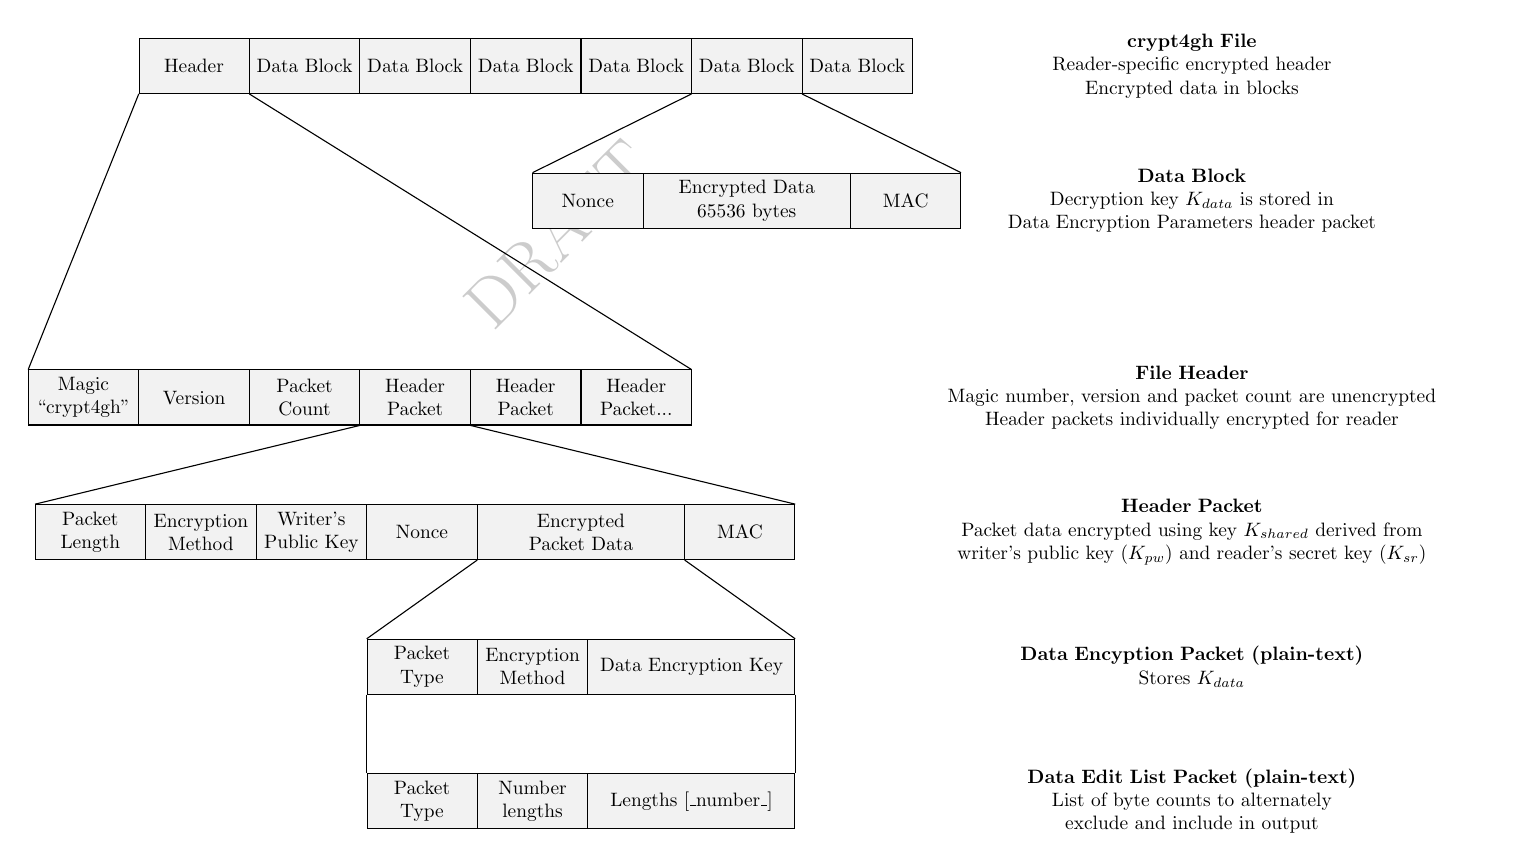
\begin{tikzpicture}[
    every node/.style={scale=0.7},
    boxes/.style={rectangle split,rectangle split parts=#1,draw,rectangle split horizontal,text width=5em,align=center,minimum height=1cm,fill=black!5,on grid},
    notes/.style={text width=20em,align=center,minimum height=1cm,on grid},
  ]
\node (file) [boxes=7] {
\nodepart{one}Header
\nodepart{two}Data Block
\nodepart{three}Data Block
\nodepart{four}Data Block
\nodepart{five}Data Block
\nodepart{six}Data Block
\nodepart{seven}Data Block
};
\node (file notes) [notes,right=of file.east] {
  \textbf{crypt4gh File} \\
  Reader-specific encrypted header \\
  Encrypted data in blocks
};

\node (data block) [boxes=3,below=1 of file.six south] {
\nodepart{one}Nonce
\nodepart[text width=10em]{two}Encrypted Data \\ 65536 bytes
\nodepart{three}MAC
};
\draw (file.five split south) to (data block.north west);
\draw (file.six split south) to (data block.north east);
\node (data block notes) at (data block -| file notes) [notes] {
  \textbf{Data Block} \\
  Decryption key $K_{data}$ is stored in \\
  Data Encryption Parameters header packet
};

\node (header) [boxes=6,below=3.5 of file.two split south] {
\nodepart{one}Magic \\ ``crypt4gh''
\nodepart{two}Version
\nodepart{three}Packet Count
\nodepart{four}Header Packet
\nodepart{five}Header Packet
\nodepart{six}Header Packet...
};
\draw (file.south west) to (header.north west);
\draw (file.one split south) to (header.north east);
\node (header notes) at (header -| file notes) [notes,text width=30em] {
  \textbf{File Header} \\
  Magic number, version and packet count are unencrypted \\
  Header packets individually encrypted for reader
};

\node (header packet) [boxes=6,below=of header.four south] {
\nodepart{one}Packet Length
\nodepart{two}Encryption Method
\nodepart{three}Writer's Public Key
\nodepart{four}Nonce
\nodepart[text width=10em]{five}Encrypted Packet Data
\nodepart{six}MAC
};
\draw (header.three split south) to (header packet.north west);
\draw (header.four split south) to (header packet.north east);
\node (header packet notes) at (header packet -| file notes) [notes,text width=30em] {
  \textbf{Header Packet} \\
  Packet data encrypted using key $K_{shared}$ derived from writer's public key ($K_{pw}$) and reader's secret key ($K_{sr}$)
};

\node (data encryption packet) [boxes=3,below=of header packet.five south] {
\nodepart{one}Packet Type
\nodepart{two}Encryption Method
\nodepart[text width=10em]{three}Data Encryption Key
};
\draw (header packet.four split south) to (data encryption packet.north west);
\draw (header packet.five split south) to (data encryption packet.north east);
\node (data encryption packet notes) at (data encryption packet -| file notes) [notes] {
  \textbf{Data Encyption Packet (plain-text)} \\
  Stores $K_{data}$
};

\node (data edit list) [boxes=3,below=of data encryption packet.south] {
\nodepart{one}Packet Type
\nodepart{two}Number lengths
\nodepart[text width=10em]{three}Lengths [\_number\_]
};
\draw (data encryption packet.south west) to (data edit list.north west);
\draw (data encryption packet.south east) to (data edit list.north east);
\node (data edit list notes) at (data edit list -| file notes) [notes] {
  \textbf{Data Edit List Packet (plain-text)} \\
  List of byte counts to alternately exclude and include in output
};
\end{tikzpicture}
\end{center}

The encrypted file structure, shown in the diagram above, consists of the following parts:

\begin{itemize}
\item A header containing: a ``magic'' string, version number and header packet count.
\begin{itemize}
\item A ``magic'' string for file type identification.
\item A version number.
\item The header packet count.
\item One or more header packets containing:
\begin{itemize}
\item The packet length in bytes.
\item The method used to encrypt the header packet data.
\item The writer's public key  ($K_{pw}$) used to encrypt the header packet data.
This is needed (along with the reader's secret key $K_{sr}$)
to calculate the shared key used to encrypt the header packet.
\item A random ``nonce'', also required for decryption.
\item The encrypted data for the header packet.
\item A MAC calculated over the encrypted header packet data.
\end{itemize}
The first item in the encrypted header packet data is a code indicating the packet type.
This is followed by type-specific data, described in section~\ref{overview:header_packet_types}.
\end{itemize}
\item The encrypted data.
This is the actual application data, stored in a sequence of blocks containing:
\begin{itemize}
\item A random ``nonce'', needed for decryption.
\item 64 kilobytes of encrypted data (the last block may contain less than this).
\item A MAC calculated over the encrypted data.
\end{itemize}
\end{itemize}

\subsection{Header Packet Types}\label{overview:header_packet_types}
There are two types of header packet:
\begin{itemize}
\item Data encryption key packets.

These describe the parameters used to encrypt one or more of the data blocks.
They contain a code indicating the type of encryption, and the symmetric key ($K_{data}$) needed to decrypt the data.

If parts of the data have been encrypted with different keys, more than one of this packet type will be present.

\item Data edit list packets.

These packets allow parts of the data to be discarded after decryption.
They can be used to avoid having to decrypt and re-encrypt files during splicing operations.

For example, a user may want to extract the blocks corresponding to Chromosome X from a CRAM file and store them
in a new file.
If the start and end points of the extract do not correspond to a 64Kbyte data block boundary, they would normally
have to decrypt all of the data blocks covering the region, discard a few bytes from the start and end, re-encrypt the
remaining data and store it in a new file.

The data edit list enables a simpler solution where the necessary encrypted data blocks are copied directly into
the new file.
On reading, the data blocks are decrypted and then the edit list is used to find out which parts of the unencrypted
data should be discarded.
\end{itemize}

\subsection{Encoding For Multiple Public/Secret Key Pairs}

It is sometimes useful to encrypt files so that they can be accessed using more than one secret key ($K_{sr}$).
For example, multiple members of a team may need to access to a file with their own key.

To allow this,
the header packet data is encrypted using each reader's public key ($K_{pr}$) and stored in a separate header packet
for each individual reader.

Where this is done, it is likely that anyone reading the file will only have the correct secret key ($K_{sr}$) for a
subset of the header packets.
Attempting to decode a header packet with the wrong key will result in a failure to verify the MAC stored in the file.
When this happens, implementations should ignore the undecodable header packet and move on to the next one.
Failing to decrypt a packet in this way SHOULD NOT cause an error to be reported;
however an error MUST be raised if, on reaching the end of the header,
it has not been possible to decrypt at least one data encryption key packet.

\section{Detailed Specification}
\subsection{Overall Conventions}
\subsubsection{Hexadecimal Numbers}
Hexadecimal values are written using the digits 0-9, and letters a-f for values 10-15.
Values are written with the most-significant digit on the left, and prefixed with "0x".

\subsubsection{Byte Ordering}
The basic data size is the byte (8 bits).
All multi-byte values are stored in least-significant byte first (``little-endian'') order.
For example, the value 1234 decimal (0x4d2) is stored as the byte stream 0xd2 0x04.

\subsubsection{Integer Types}
Integers can be either signed or unsigned.
Signed values are stored in two's complement form.

\subsubsection{Multi-byte Integer Types}
\begin{center}
\begin{tabular}{l l l l}
\hline
\textbf{Name} & \textbf{Byte Ordering} & \textbf{Integer Type} & \textbf{Size (bytes)} \\
\hline
byte & & unsigned & 1 \\
le\_int32 & little-endian & signed & 4 \\
le\_uint32 & little-endian & unsigned & 4 \\
le\_int64 & little-endian & signed & 8 \\
le\_uint64 & little-endian & unsigned & 8 \\
le\_uint96 & little-endian & unsigned & 12 \\
\end{tabular}
\end{center}

\subsubsection{Structures}
Structure types may be defined (in C-like notation) for convenience.

\begin{verbatim}
struct demo {
  byte string[8];
  le_int32 number1;
  le_uint64 number2;
};
\end{verbatim}

When structures are serialised to a file, elements are written in the given order with no padding between them.
The above structure would be written as twenty bytes - eight for the array `string', four for the integer `number1',
and eight for the integer `number2'.

\subsubsection{Enumerated Types}
Enumerated types may only take one of a given set of values.
The data type used to store the enumerated value is given in angle brackets after the type name.
Every element of an enumerated type must be assigned a value.
It is not valid to compare values between two enumerated types,
except to compare for (in)equality.

\begin{verbatim}
enum Animal<le_uint32> {
  cat    = 1;
  dog    = 2;
  rabbit = 3;
};
\end{verbatim}

\subsubsection{Variants}
Parts of structures may vary depending on information available at the time of decoding.
Which variant to use is selected by an enumerated type.
There must be a case for every possible enumerated value.
Cases have limited fall-through.
Consecutive cases with no fields in between all contain the same fields.

\begin{verbatim}
struct AnimalFeatures {
  select (enum Animal) {
    case cat:
    case dog:
      le_uint32 hairyness;
      le_uint32 whisker_length;

    case rabbit:
      le_uint32 ear_length;
  };
};
\end{verbatim}

For the `cat' and `dog' cases, `struct AnimalFeatures' is eight bytes long and contains two unsigned four-byte
little-endian values.
For the `rabbit' case it is four bytes long and contains a single four-byte little-endian value.

If the cases are different lengths (as above), then the size of the overall structure depends on the variant chosen.
There is NO padding to make the cases the same length unless it is explicitly defined.

\subsection{Header}

The file starts with a header, with the following structure:

\begin{verbatim}
struct Header {
  byte                          magic_number[8];
  le_uint32                     version;
  le_uint32                     header_packet_count;
  Encrypted_header_packet       header_packets[header_packet_count]
};
\end{verbatim}

The \kw{magic\_number} is the ASCII representation of the string ``crypt4gh''.

The version number is stored as a four-byte little-endian unsigned integer.
The current version number is 1.

The current byte representation of the magic number and version is:
\begin{verbatim}
0x63 0x72 0x79 0x70 0x74 0x34 0x67 0x68 0x01 0x00 0x00 0x00
============= magic_number============= ===== version =====
\end{verbatim}

\kw{header\_packet\_count} is the number of header packets that follow.

\subsubsection{Header Packets}\label{header:encryption}

The header packets are defined as:

\begin{verbatim}
enum Header_encryption_method<le_uint32> {
  X25519_chacha20_ietf_poly1305 = 0;
};

struct Header_packet {
  le_uint32                           packet_length;
  Header_encryption_method<le_uint32> packet_encryption;

  select (packet_encryption) {
    case X25519_chacha20_ietf_poly1305:
      byte   writer_public_key[32];
      byte   nonce[12];
  };

  byte encrypted_payload[];

  select (packet_encryption) {
    case X25519_chacha20_ietf_poly1305:
      byte MAC[16];
  };
};
\end{verbatim}

\kw{packet\_length} is the length of the entire header packet (including the \kw{packet\_length} itself).
To prevent packet types from being guessed by looking at the size, it is permitted for the \kw{packet\_length} to be
longer than strictly needed to encode all of the packet data.
Any remaining space after the actual data should be padded in a suitable manner (for example by setting it to zero)
and encrypted.

\kw{packet\_encryption} is the encryption method used for this header packet.

\kw{writer\_public\_key} ($K_{pw}$) and \kw{nonce} are parameters needed to decrypt the \kw{encrypted\_payload} in the
packet.

\kw{encrypted\_payload} is the encrypted part of the header packet, for which the plain-text is described below.

\kw{MAC} is a message authentication code calculated over the encrypted data.

Implementations should ignore any header packets that they cannot decrypt successfully, as these may have
been intended for a different reader.

\subsubsection{Header packet encrypted payload}

The \kw{encrypted\_payload} part of the header packet contains the following plain-text:

\begin{verbatim}
enum Header_packet_type<le_uint32> {
  data_encryption_parameters = 0;
  data_edit_list = 1;
};

enum Data_encryption_method<le_uint32> {
  chacha20_ietf_poly1305 = 0;
};

struct Encrypted_header_packet {
  Header_packet_type<le_uint32> packet_type;

  select (packet_type) {
    case data_encryption_parameters:
      enum Data_encryption_method<le_uint32>  data_encryption_method;
      select (data_encryption_method) {
        case chacha20_ietf_poly1305:
          byte  data_key[32];
      };

    case data_edit_list:
      le_uint32 number_lengths;
      le_uint64 lengths[number_lengths];
  };
};
\end{verbatim}

\kw{packet\_type} defines what sort of data packet this is.

\subsubsection{data\_encryption\_parameters packet}\label{header:data_encryption_parameters}

This packet contains the parameters needed to decrypt the data part of the file.

\kw{data\_encryption\_method} is an enumerated type that describes the type of encryption used.

\kw{data\_key} is the symmetric key $K_{data}$ used to decode the data section.

To allow parts of the data to be encrypted with different $K_{data}$ keys,
more than one of this packet type may be present.
If there is more than one, the \kw{data\_encryption\_method} MUST be the same for all of them to prevent problems
with random access in the encrypted file.

\subsubsection{data\_edit\_list packet}

This packet contains a list of edits that should be applied to the plain-text data following decryption.

\kw{number\_lengths} is the number of items in the \kw{lengths} array.

\kw{lengths} is an array of byte counts.

Application of the edit list to the plain-text is described in section~\ref{data:edit_list}.

It is not permitted to have more than one edit list.
If more than one edit list is present, the file SHOULD be rejected.

\subsection{Header packet encryption}

\subsubsection{X25519\_chacha20\_ietf\_poly1305 Encryption}~\label{header:X25519}

This method uses Elliptic Curve Diffie-Hellman key exchange with additional hashing to generate a shared
key ($K_{shared}$).
$K_{shared}$ is then used along with a randomly-generated nonce to encrypt the header packet data using the
ChaCha20-IETF-Poly1305 construction.
The elliptic curve algorithm used is X25519, described in section 5 of \cite{RFC7748}.

Encryption requires the writer's public and secret keys ($K_{pw}$ and $K_{sw}$), the reader's public key ($K_{pr}$)
and a nonce ($N$).

The nonce is a unique initialisation vector.
In ChaCha20-IETF-Poly1305 it is 12 bytes long.
This value MUST be unique for each packet encrypted with the same reader's and writer's keys.
The best way to ensure this is to generate a value with a cryptographically-secure random number generator.

The secret keys MUST be generated using a cryptographically-secure random number generator.
The corresponding public keys are derived using the method in section 6.1 of \cite{RFC7748}.

$K_p = X25519(K_s, 9)$

The writer's secret key and the reader's public key are used to generate a Diffie-Hellman shared key as described in
section 6.1 of \cite{RFC7748}.

$K_{dh} = X25519(K_{sw}, K_{pr})$

As the X25519 algorithm does not produce a completely uniform bit distribution,
and many possible $(K_{sw}, K_{pr})$ pairs can produce the same output,
the Diffie-Hellman key is hashed along with the two public keys to produce the final shared key.
The hash function used to do this is Blake2b, as described in \cite{RFC7693}.

$K_{shared} = Blake2b(K_{dh} || K_{pr} || K_{pw})$

As ChaCha20 uses a 32-byte key, only the first 32 bytes of $K_{shared}$ are used; the rest are discarded.

The header packet type, data and any padding is then encrypted using the method described in the
chacha20\_ietf\_poly1305 Encryption section~\ref{data:chacha20_encryption}.
Note that header packets are not segmented; they are always encrypted in a single block.

Finally, the packet length, encryption type, writer's public key $K_{pw}$,
the nonce $N$ and the encrypted header packet data are combined to make the header packet.

For extra security, writers MAY choose to discard the writer's secret key $K_{sw}$ after use.
Due to the symmetry of the Diffie-Hellman algorithm, the holder of either secret key can regenerate the shared
key as long as the other public key is known.
Deleting the writer's key $K_{sw}$ ensures only the holder of the reader's secret key $K_{sr}$ can decode the header
packet.
As long as the writer uses randomly-generated keys, it also makes accidental nonce reuse very unlikely.

\subsubsection{X25519\_chacha20\_ietf\_poly1305 Decryption}

To decrypt the header packet, the reader obtains the writer's public key $K_{pw}$ and the nonce from the beginning
of the packet.
Also needed are the reader's public and secret keys ($K_{pr}$ and $K_{sr}$).

The Diffie-Helman key is obtained using:

$K_{dh} = X25519(K_{sr}, K_{pw})$

This is then hashed to obtain the shared key (again only the first 32 bytes are retained):

$K_{shared} = Blake2b(K_{dh} || K_{pr} || K_{pw})$

The resulting key $K_{shared}$ and nonce $N$ are then used to decrypt the remainder of the packet.

If the header packet was intended for a different reader, the reader will be unable to decode the header packet
as the Poly1305 MAC will be incorrect.
This should not be considered an error.

\subsubsection{Reading the header}

The reader should check that the \kw{magic\_number} and \kw{version} in the header match the expected values.

It should then attempt to decode all of the header packets, ignoring any that do not decrypt successfully
(detected by a failure to verify the MAC).
At the end of this process the reader should have decoded at least one \kw{data\_encryption\_parameters} packet.
If no such packet was decoded, it SHOULD report an error.
If more than one is present, they should all have the same \kw{data\_encryption\_method}, otherwise the reader
SHOULD report an error.
The reader should store all of the keys that it has decoded in a list for use when decoding the encrypted data section.

If a \kw{data\_edit\_list} packet is found, the reader should store it for use while processing the data blocks.
If more than one \kw{data\_edit\_list} packet is present, the file SHOULD be rejected.

\subsection{Encrypted Data}\label{data:encryption}
\subsubsection{chacha20\_ietf\_poly1305 Encryption}\label{data:chacha20_encryption}

ChaCha20 is a stream cipher which maps a 256-bit key, nonce and counter to a 512-bit key-stream block.
In IETF mode the nonce is 96 bits long and the counter is 32 bits.
The counter starts at 1, and is incremented by 1 for each successive key-stream block.
The cipher-text is the plain-text message combined with the key-stream using the bit-wise exclusive-or operation.

Poly1305 is used to generate a 16-byte message authentication code (MAC) over the cipher-text.
As the MAC is generated over the entire cipher-text it is not possible to authenticate partially decrypted data.

ChaCha20 and Poly1305 are combined using the AEAD construction described in section 2.8 of \cite{RFC8439}.
This construction allows additional authenticated data (AAD) to be included in the Poly1305 MAC calculation.
For the purposes of this format, the AAD is zero bytes long.

\subsubsection{Segmenting the input}

To allow random access without having to authenticate the entire file, the plain-text is divided into 65536-byte
(64KiB) segments.
If the plain-text is not a multiple of 64KiB long, the last segment will be shorter.
Each segment is encrypted using the method defined in the header.
The nonce used to encrypt the segment is then stored, followed by the encrypted data, and then the MAC.

\begin{verbatim}
struct Segment {
  select (method) {
    case chacha20_ietf_poly1305:
      byte    nonce[12];
      byte[]  encrypted_data;
      byte    mac[16];
  };
};
\end{verbatim}

The addition of the \kw{nonce} and \kw{mac} bytes will expand the data slightly.
For chacha20\_ietf\_poly1305, this expansion will be 28 bytes, so a 65536 byte plain-text input will become a 65564
byte encrypted and authenticated cipher-text output.

\section{Decryption}

\subsection{chacha20\_ietf\_poly1305 Decryption}

The cipher-text is decrypted by authenticating and decrypting the segment(s) enclosing the requested byte range $[P;Q]$,
where $P<Q$.
For a range starting at position $P$, the location of the segment \kw{seg\_start} containing that position must
first be found.
For the chacha20\_ietf\_poly1305 method, when no edit list is in use, this can be done using the formula:

\begin{verbatim}
seg_start = header_len + floor(P/65536) * 65564
\end{verbatim}

For an encrypted segment starting at position \kw{seg\_start}, the nonce, then the 65536 bytes of cipher-text
(possibly fewer of it was the last segment), and finally the MAC are read.

An authentication tag is calculated over the cipher-text from that segment, and bit-wise compared to the MAC.
The cipher-text is authenticated if and only if the tags match.
If more than one key ($K_{data}$) was included in the header,
each should be tried in turn until either one authenticates correctly or no keys are left to try.
An error MUST be reported if the cipher-text is not authenticated.

The key $K_{data}$ and nonce $N$ are then used to decrypt the cipher-text for the segment, returning the plain-text.
Successive segments are decrypted, until the segment containing position $Q$ is reached.
The plain-text segments are concatenated to form the resulting output, discarding $P \mathbin{\%} 65536$ bytes from
the beginning of the first segment and retaining $Q \mathbin{\%} 65536$ bytes of the last one.

If more than one key ($K_{data}$) is in use,
readers can speed up decryption by trying the previous successful key first when attempting to authenticate each block.
However, this does open up a possible timing attack where an observer watching the decoding process can find
out where key changes occur due to the extra time needed to select the new key at these points.
If this is unacceptable, readers could either try each key for every block (although this may still be vulnerable
to timing attacks which try to detect which key was successful); or simply insist that only one key is used for
the whole file.

\subsection{Edit List}\label{data:edit_list}

The edit list is designed to assist splicing of encrypted files (for example to remove parts that are not needed
for later analysis) without having to decrypt and re-encrypt the entire file.
It is only possible to splice crypt4gh files at the 64K encryption block boundaries.
The edit list can be used to work around this limitation by describing which parts of the unencrypted blocks
should be discarded to give the final desired plain-text.

The following algorithm describes how to apply the edit list $edlist$ to unencrypted text $input$ to return
the desired edited plain-text.
In this algorithm, function \textsc{IsEmpty} returns true if a list is empty and false if not.
Function \textsc{RemoveFirst} removes the first item from a list and returns it.
\textsc{length} returns the length of a string.
\textsc{substr} returns part of a string from a given zero-based position and with a given length (or shorter if the
requested part extends beyond the end of the input string).
\textsc{StringConcatenate} returns the string concatenation of its input parameters in order from left to right.

\begin{algorithmic}[1]
\Function{ApplyEditList}{$edlist,\ input$}
\If{\Call{IsEmpty}{edlist}}
  \State \textbf{return} $input$\Comment{Trivial case with no edit list}
\EndIf
\settowidth{\maxwidth}{output}
\State \algalign{output}{\gets} ``''\Comment{Initial output is empty}
\State \algalign{pos}{\gets} $0$\Comment{Current position in the unedited plain-text}
\State \algalign{len}{\gets} \Call{length}{input}\Comment{Length of input string}
\Repeat
  \settowidth{\maxwidth}{discard}
  \State \algalign{discard}{\gets} \Call{RemoveFirst}{edlist}\Comment{Pull number of bytes to discard from list}
  \State \algalign{pos}{\gets} $pos + discard$
  \If{\Call{IsEmpty}{edlist}}
     \settowidth{\maxwidth}{output}
     \State \algalign{part}{\gets} \Call{substr}{$input, pos, len - pos$}\Comment{Append the remainder of $input$}
     \State \algalign{output}{\gets} \Call{StringConcatenate}{$output,\ part$}
  \Else
     \settowidth{\maxwidth}{output}
     \State \algalign{keep}{\gets} \Call{RemoveFirst}{edlist}\Comment{Pull number of bytes to keep from the list}
     \State \algalign{part}{\gets} \Call{substr}{$input, pos, keep$}\Comment{Append this part to $output$}
     \State \algalign{output}{\gets} \Call{StringConcatenate}{$output,\ part$}
     \State \algalign{pos}{\gets} $pos + keep$
  \EndIf
\Until{\Call{IsEmpty}{edlist}}
\State \textbf{return} $output$
\EndFunction
\end{algorithmic}

\subsubsection{Example}

Imagine that for some reason we have made an encrypted copy of ERR2436651.
\footnote{The data for this example comes from \url{ftp://ftp.sra.ebi.ac.uk/vol1/run/ERR243/ERR2436651/}.}

We would like to make a new encrypted file including just the data aligned to ChrII,
without having to decrypt and re-encrypt the desired data.
The new file will need to include the following items (note that byte ranges are zero-based inclusive):

\begin{enumerate}
\item A crypt4gh header containing the keys needed to decrypt the file.
\item The CRAM header (plain-text bytes 0 to 7852).
\item ChrII data (plain-text bytes 145110 to 453038).
\item The CRAM end-of-file block (plain-text bytes 5485074 to last byte of file at 5485111).
\end{enumerate}

None of these byte ranges align with 64K boundaries.
To avoid the need to decrypt and re-encrypt the data,
an edit list can be added to the crypt4gh header and the byte ranges are expanded to complete encrypted blocks.
After this the list of items to send will be:

\begin{enumerate}
\item A crypt4gh header containing the keys needed to decrypt the file and an edit list.
\item The CRAM header (plain-text bytes 0 to 65535).
\item ChrII data (plain-text bytes 131072 to 458751).
\item The CRAM end-of-file block (plain-text bytes 5439488 to last byte of file at 5485111).
\end{enumerate}

These segments will be concatenated to make the new file,
so in this case to obtain the desired data the edit list will contain the values:
\begin{center}
$[0, 7853, 71721, 307929, 51299, 38]$
\end{center}

Which means:

\begin{itemize}
\item Discard zero bytes from the start.
\item Keep 7853 bytes (the CRAM header).
\item Discard 57683 bytes (following the CRAM header) + 14038 bytes (before ChrII data) = 71721 bytes in total.
\item Keep 307929 bytes (ChrII data).
\item Discard 5713 bytes (following ChrII) + 45586 bytes (before the EOF block) = 51299 bytes in total.
\item Keep 38 bytes (EOF block).
This could actually be left out as it extends all the way to the end of the file.
\end{itemize}

\section{Security Considerations}
\subsection{Threat Analysis}
This format is primarily designed to protect files at rest and in transport from accidental disclosure.
Attackers are assumed to have read access to encrypted files.
Even if this is the case,
it should not be possible to decrypt the file without access to the reader's secret key ($K_{sr}$).

Some file formats use supplementary files, for example external indices.
In some cases it may be possible to deduce information about the data file from the supplementary one.
For example, it is usually trivial to determine gender from a BAM index,
and it may also be possible to detect certain other genetic conditions.
Where the main data file needs to be encrypted, such supplementary files MUST be encrypted as well.

While key management is out of scope for this document,
it should be noted that it is important that attackers are not able to access secret keys.
Implementations MUST ensure that secret keys are kept in a secure manner.

Attackers with write access to files will not be able to make changes to individual blocks as
(without access to the decryption key) they will not be able to calculate the correct MAC on the new version.
Such an attacker can, however, make block-level changes such as removing or reordering blocks.
An attacker with access to the reader's public key ($K_{pr}$) will also be able to add entire blocks by inserting a new
data\_encryption\_parameters packet in the header, and using the key stored in it to encrypt the new block.

It is expected that files using this format will be decrypted in memory for processing.
There is a risk of data being leaked either directly or through a side-channel (many of which are difficult to defend
against).
It is very likely that attackers who gain access to machines analysing data in encrypted files will be able
to make deductions about the file contents, or in the worst case either extract the entire decrypted file or
obtain the decryption keys.

Implementations SHOULD use cryptographic libraries hardened against common side-channel (e.g. timing) attacks.
Implementations MUST keep secret material as safe as possible.
For example, keys should ideally be locked into memory to avoid them being paged to a swap file.
Keys should also be securely erased as soon as they are no longer needed.
Any intermediate files written out during processing SHOULD be encrypted.

Deployments MUST take precautions to prevent attackers from accessing data while it is processed.
Note that the following list is not exhaustive.
\begin{itemize}
\item Software MUST be kept up to date for security patches.
\item Data should not be processed on machines shared by more than one user.
\item Local file systems and swap partitions should be encrypted.
\item Debugging interfaces (for example ptrace) should be disabled.
\item Machines should not be running any unnecessary processes or services.
\item Firewall rules should be used to restrict network access to only sites needed for processing the data.
\item Users should avoid running processes like web browsers that can run arbitrary code downloaded from the Internet
(even if the code is run in a sand-box environment) on a machine where encrypted data is being processed.
\end{itemize}

\subsection{Selection of Keys}
The security of the format depends on attackers not being able to guess secret keys ($K_{sr}$ and $K_{sw}$)
or the data encryption key ($K_{data}$).
The keys MUST be generated using a cryptographically-secure pseudo-random number generator.
This makes the chance of guessing a key vanishingly small.

\subsection{Nonce selection}
All header packets encrypted with the same combination of writer's secret key ($K_{sw}$)
and reader's public key ($K_{pr}$) MUST use a unique nonce.
If the writer uses the same secret key ($K_{sw}$) for more than one file then all nonces MUST be unique across all
files made with that key.
As each file will only include a few header packets this restriction can be fulfilled by generating each nonce
using a cryptographically-secure random number generator.
If the writer uses a randomly-generated $K_{sw}$ for each file, or even each header packet, the risk of nonce reuse in
the header is almost completely eliminated.

All data segments encrypted with the same key MUST use a unique nonce.
One way to ensure this is to choose a random starting point and then use a counter or linear-feedback shift
register to generate the nonce for each segment.
This method guarantees a unique value even for very long files.

For a 96-bit nonce, it may be acceptable to generate each one using a cryptographically-secure pseudo-random number
generator.
Care should be taken to ensure that the random number generator is capable of generating a long enough stream
of unique values.
Due to the birthday problem, this method will have a non-zero (but very small) probability of failing.
For example, a file of 24 Terabytes will have a reused nonce with probability of approximately $10^{-12}$

\subsection{Message Forgery}
Using ChaCha20-IETF-Poly1305 authenticates the content of each header packet and each segment of the encrypted
cipher-text.
It does not protect against the addition or removal of header packets, or the addition, removal or rearrangement
of data segments.
crypt4gh files are not signed, so there is no direct way to prove that a file was created by a given writer.

\subsection{No File Updates Permitted}
Implementations MUST NOT update encrypted files.
Once written, a section of the file must never be altered.

\bibliographystyle{abstract}

\begin{thebibliography}{XXXXXXX}

% Normative references
\subsection{Normative References}

\bibitem[RFC2119]{RFC2119}
  Bradner, S.,\\
  \emph{"Key words for use in RFCs to Indicate Requirement Levels", BCP 14, RFC 2119},\\
  \url{https://www.rfc-editor.org/info/rfc2119},\\
  March 1997

\bibitem[RFC7693]{RFC7693}
  Saarinen, M.J., Aumasson, J.P.\\
  \emph{"The BLAKE2 Cryptographic Hash and Message Authentication Code (MAC)", RFC7693},\\
  \url{https://tools.ietf.org/html/rfc7693},\\
  November 2015

\bibitem[RFC7748]{RFC7748}
  A. Langley, Google, M. Hamburg, Rambus Cryptography Research, S. Turner, sn3rd,\\
  \emph{"Elliptic Curves for Security", RFC7748},\\
  \url{https://tools.ietf.org/html/rfc7748},\\
  January 2016

\bibitem[RFC8032]{RFC8032}
  S. Josefsson, SJD AB, I. Liusvaara,\\
  \emph{"Edwards-Curve Digital Signature Algorithm (EdDSA)", RFC8032},\\
  \url{https://tools.ietf.org/html/rfc8032},\\
  January 2017

\bibitem[RFC8439]{RFC8439}
  Y. Nir, Dell EMC, A. Langley, Google, Inc.,\\
  \emph{"ChaCha20 and Poly1305 for IETF Protocols", RFC8439},\\
  \url{https://tools.ietf.org/html/rfc8439},\\
  June 2018

% Informational references
\subsection{Informational References}

\bibitem[RFC4880]{RFC4880}
  Callas, J., PGP Corporation, Donnerhacke, L., IKS GmbH, Finney, H., PGP Corporation, Shaw, D., Thayer, R.,\\
  \emph{"OpenPGP Message Format", RFC 4880},\\
  \url{https://www.rfc-editor.org/info/rfc4880},\\
  November 2007.

\bibitem[RFC8446]{RFC8446}
  Rescorla, E.,\\
  \emph{"The Transport Layer Security (TLS) Protocol Version 1.3", RFC 8446},\\
  \url{https://www.rfc-editor.org/info/rfc8446},\\
  August 2018.

\bibitem[RFC8551]{RFC8551}
  Schaad, J., August Cellars, Ramsdell, B., Brute Squad Labs, Inc., Turner, S.,\\
  \emph{"Secure/Multipurpose Internet Mail Extensions (S/MIME) Version 4.0 Message Specification", RFC 8551},\\
  \url{https://www.rfc-editor.org/info/rfc8551},\\
  April 2019.

\bibitem[AE LIMITS]{AE LIMITS}
  Luykx, A., Paterson, K.,\\
  \emph{"Limits on Authenticated Encryption Use in TLS"},\\
  \url{http://www.isg.rhul.ac.uk/~kp/TLS-AEbounds.pdf},
  August 2017.

\bibitem[Curve25519]{Curve25519}
  Bernstein, Daniel J.,\\
  \emph{"Curve25519: New Diffie-Hellman Speed Records"},\\
  \url{https://doi.org/10.1007%2F11745853_14},\\
  2006.

\bibitem[SafeCurves]{SafeCurves}
  Bernstein, Daniel J., Lange, Tanja,\\
  \emph{"SafeCurves: choosing safe curves for elliptic-curve cryptography."},\\
  \url{https://safecurves.cr.yp.to},\\
  accessed 22 July 2019.

\bibitem[Blake2]{Blake2}
  Aumasson, J-P., Neves, S., Wilcox-O’Hearn, Z., Winnerlein, C.,\\
  \emph{"BLAKE2: simpler, smaller, fast as MD5"},\\
  \url{https://eprint.iacr.org/2013/322.pdf},\\
  2013.

\bibitem[Post-Quantum]{Post-Quantum}
  Alagic, G., Alperin-Sheriff, J., Apon, D., Cooper, D., Dang, Q., Miller, C., Moody, D., Peralta, R., Perlner, R., Robinson, A., Smith-Tone, D, Liu, Y-K.,\\
  \emph{"Status Report on the First Round of the NIST Post-Quantum Cryptography Standardization Process"},\\
  \url{https://doi.org/10.6028/NIST.IR.8240},\\
  January 2019.

\bibitem[htsget]{htsget}
  Kelleher, J., Lin, M., Albach, C. H., Birney, E., Davies, R., Gourtovaia, M., Glazer, D., Gonzalez, C. Y., Jackson, D. K., Kemp, A., Marshall, J., Nowak, A., Senf, A., Tovar-Corona, J. M., Vikhorev, A., Keane, T. M., GA4GH Streaming Task Team
  \emph{"htsget: a protocol for securely streaming genomic data"}
  \url{https://doi.org/10.1093/bioinformatics/bty492}
  June 2018.

\end{thebibliography}

\appendix
\section{Rationale}

Using authenticated encryption in individual segments mirrors solutions like Transport Layer
Security (TLS) as described in~\cite{RFC8446} and prevents undetected modification of segments.
Dividing the file into fixed-size (except at the end) blocks allows random-access into the encrypted file.
The format is also designed to allow streaming reads and writes;
in particular when writing no more than 64 Kbytes of plain-text needs to be known at any point.

While the standard allows for multiple encryption methods, only one choice is currently allowed.
This simplifies implementations while allowing the current choice to be replaced in a future revision if it is found
to have any vulnerabilities.
The criteria for choosing encryption methods included having strong security guarantees, good library support
and being used in other common standards like TLS version 1.3.

\subsection{Symmetric Encryption}

For symmetric encryption, the main candidates for authenticated encryption were AES-GCM and ChaCha20-Poly1305.
Both have good security guarantees, and thanks to their use in TLS 1.3 both have good library support.
ChaCha20-Poly1305 was chosen because it allows much longer files to be encrypted.
See~\cite{AE LIMITS} for a comparison although note that our ``messages'' are $2^{16}$ bytes long,
while the figures in the paper are for $2^{14}$ bytes.

There are three common ChaCha20-Poly1305 constructions original, ChaCha20-IETF-Poly1305, and XChaCha20-Poly1305.
The main differences are the length of the nonce and the maximum message size allowed using a single nonce.
ChaCha20-IETF-Poly1305 was chosen because it has the best library support thanks to its use in Internet Engineering
Task Force protocols and the nonce length allows a very large number of messages to be encrypted under a single key.
The message length restriction of ChaCha20-IETF-Poly1305 ($64*2^{32}-64$ bytes) is not a problem as our ``messages''
are at most 64 Kbytes long.

\subsection{Public-key Algorithm}

For public-key encryption Elliptic Curve Diffie-Hellman using X25519 was chosen.
Elliptic Curve Diffie-Hellman is faster and uses smaller keys than methods such as RSA or traditional Diffie–Hellman.
X25519 is based on Curve25519 which allows fast implementations, has good security properties~\cite{Curve25519}
and has been constructed to avoid a number of possible implementation problems~\cite{SafeCurves}.
X25519 is used in TLS version 1.3, S/MIME 4.0~\cite{RFC8551} and many other protocols, and has good library support.

X25519 is used to generate a shared key.
While this key could be used on its own, its properties are not ideal because many secret/public key pairs can
generate the same key and the bit distribution across the key is not completely uniform.
To enhance the key, it is concatenated with the two public keys used in the key exchange and then passed through
a secure hash function.
The chosen hash function (Blake2b) has good library support,
is faster than SHA-2 and has similar security to that of SHA-3~\cite{Blake2}.

The generated shared key $K_{shared}$ is used as the secret material for symmetric encryption of the header packet data.
As it is already used for encrypting the data blocks, the method chosen for this is ChaCha20-IETF-Poly1305.

Like other ECDH schemes, X25519 is not resistant to attack using a quantum computer.
At the time of writing, quantum-computing resistant algorithms are undergoing standardisation~\cite{Post-Quantum}.
A future revision of this specification will add quantum-computing resistant algorithms once this process
is complete and a suitable replacement becomes widely available.

\subsection{Other Considerations}

This specification provides no way of authenticating files by signing them.
Implementing such a scheme would also involve creating infrastructure for validating the generated signatures.
This was deemed to be beyond the requirements of the format.
If authentication is required, the encrypted file can be signed separately using an existing digital signature scheme,
for example OpenPGP~\cite{RFC4880}.

Dividing the header into individually encrypted ``packets'' allows the data to be decrypted by more than one key,
and also allows parts of the data to be encrypted using different keys.
The former allows files to be accessed by more than one user without them having to share keys.
The latter allows for selective access to parts of a file - although this only works for random access.
Trying to stream such a file will likely result in an error when the reader reaches a part for which it does not have
a suitable key.

The data edit list header packets were added to make it easier to serve encrypted files using htsget~\cite{htsget}.
Htsget is designed to serve parts of a genomic data file in response to a web request,
Htsget servers return a list of file parts that should be downloaded and concatenated to give the desired result.
Most of these parts can simply be served directly from a static file store, allowing the htsget back-end to efficiently
handle a large number of requests.

Allowing htsget to serve encrypted files would be beneficial as the data in the static file store can be stored in
an encrypted form.
For efficiency (and better security),
the htsget server would want to avoid decrypting and re-encrypting the file blocks when serving them.
This is possible,
but there is a complication when the requested data does not align to the 64 Kbyte encrypted block boundaries.
The partial block would need to be rewritten so that it starts in the correct location.
As all encrypted blocks except the last must contain exactly 64 Kbytes, this would pull in data from the next block,
which would also have to be rewritten and so on until the end of the file.
This would essentially involve decrypting and re-encrypted the entire region.

A more efficient solution, which is enabled by the data edit list, is to serve the entire misaligned block and
include information about the parts that should be discarded in the header.
The client then discards the unwanted data after decryption.
Being able to serve the encrypted data directly and avoiding the need to handle plain-text should more than
compensate for the minor inefficiency of serving slightly more data (at most 131070 bytes per region) than requested.
The added complication of supporting edit lists in client code is also fairly minor compared to other
necessary parts of the format (for example key handling).

\end{document}

\title{GA4GH File Encryption Standard}
\date{\headdate}
\maketitle
\begin{quote}\small
The master version of this document can be found at
\url{https://github.com/samtools/hts-specs}.\\
This printing is version~\commitdesc\ from that repository,
last modified on the date shown above.
\end{quote}
\vspace*{1em}

\begin{abstract}
This document describes the format for Global Alliance for Genomics and Health (GA4GH) encrypted files.
Encryption helps to prevent accidental disclosure of confidential information.
Allowing programs to directly read and write data in an encrypted format reduces the chance of such disclosure.
The format described here can be used to encrypt any underlying file format.
It also allows for seeking on the encrypted data.
In particular indexes on the plain text version can also be used on the encrypted file without modification.
\end{abstract}
\newpage
\tableofcontents
\newpage
\section{Introduction}
\subsection{Purpose}
By its nature, genomic data can include information of a confidential nature about the health of individuals.
It is important that such information is not accidentally disclosed.
One part of the defence against such disclosure is to, as much as possible, keep the data in an encrypted format.

This document describes a file format that can be used to store data in an encrypted state.
Existing applications can, with minimal modification, read and write data in the encrypted format.
The choice of encryption also allows the encrypted data to be read starting from any location, facilitating indexed
access to files.

The format has the following properties:

\begin{itemize}
\item Confidentiality

Data stored in the file is only readable by holders of the correct secret decryption key.
The format does not hide the length of the encrypted file, although it is possible to pad some file structures to
obscure the length.

\item Integrity

Data is stored in a series of 64 kilobyte blocks, each of which includes a message authentication code (MAC).
Attempts to change the data in a block will make the MAC invalid; it is not possible to recalculate the MAC without
knowing the key used to encrypt the file.

The format only protects the contents of each individual block.
It does not protect against insertion, removal, or reordering of entire blocks.

\item Authentication

The format does not provide any way of authenticating files.
\end{itemize}

\subsection{Requirements}
The key words ``MUST'', ``MUST NOT'', ``REQUIRED'', ``SHALL'', ``SHALL NOT'', ``SHOULD'', ``SHOULD NOT'',
``RECOMMENDED'', ``MAY'', and ``OPTIONAL'' in this document are to be interpreted as described in \cite{RFC2119}.

\subsection{Terminology}
\begin{description}
\item[cipher-text]~\\
The encrypted version of the data.

\item[plain-text]~\\
The unencrypted version of the data.

\item[symmetric encryption]~\\
Encryption where the writer and reader use the same key.

\item[public-key encryption]~\\
Encryption where a non-secret public key is used to encrypt data and a different secret private key is used to decrypt.

\item[Elliptic-curve cryptography (ECC)]~\\
An approach to public-key cryptography based on the algebraic structure of elliptic curves over finite fields.

\item[Diffie-Hellman]~\\
A method of generating a shared cryptographic key, used for public-key encryption.

\item[Elliptic-curve Diffie-Hellman (ECDH)]~\\
A variant of Diffie-Hellman using elliptic curve cryptography.

\item[Curve25519]~\\
A widely used FIPS-140 approved ECC algorithm not encumbered by any patents \cite{RFC7748}.

\item[X25519]~\\
An elliptic-curve Diffie-Hellman algorithm using Curve25519.

\item[ChaCha20-IETF-Poly1305]~\\
ChaCha20 is a symmetric stream cipher built on a pseudo-random function that gives the advantage that one can
efficiently seek to any position in the key stream in constant time.
It is not patented.
Poly1305 is a cryptographic message authentication code (MAC).
It can be used to verify the data integrity and the authenticity of a message \cite{RFC8439}.

\item[nonce]~\\
A number that is used only once.
Such numbers are used to set the initial state in cryptographic constructions.
It is important that they are not reused as it is possible for attackers to learn information about data blocks that
have been encrypted using the same key and nonce.
In the worst case this can lead to a complete break-down of the security of the encryption.

\item[MAC]~\\
Message authentication code.
A MAC is a short tag generated by an algorithm which takes a message and a secret key as inputs.
To be secure, it should be computationally infeasible to generate the same MAC without knowing the secret key.
A holder of the secret key can run a verification algorithm on the MAC to ensure with high probability that the
message has not been altered after the MAC was generated.

\item[magic string]~\\
A byte pattern that can be used for file format identification.
Usually put at the start of a file so that software can probe the first few bytes to determine what sort of file
it is reading.

\end{description}

\section{Encrypted Format Overview}

\subsection{Keys}

A number of cryptographic keys are required by the format.
The type and function of each key is listed here,
along with symbols ($K_x$ where $_x$ is the key type) used to refer to the key in the rest of this specification.

\subsubsection{Asymmetric Keys}

This specification uses the term ``secret key'' rather than ``private key'' so that the symbol $K_s$ can be used
for secret keys and $K_p$ for public keys.

\begin{description}

\item{Reader's secret key ($K_{sr}$)}~\\
This key is used by the reader when decrypting header packets and should be kept private.
It is generated using a cryptographically-secure random number.

\item{Reader's public key ($K_{pr}$)}~\\
This key is passed to the writer so that they can encrypt header packets (section~\ref{header:encryption}) for the
reader.
It is derived from $K_{sr}$ (see section~\ref{header:X25519}).

\item{Writer's secret key ($K_{sw}$)}~\\
This key is used by the writer to encrypt header packets.
It should either be kept private, or deleted after use.
It is generated using a cryptographically-secure random number.

\item{Writer's public key ($K_{pw}$)}~\\
This key is included in the header packet (section~\ref{header:encryption}) so that the reader can use it to
derive the shared key ($K_{shared}$, see below) needed to decrypt header packet data.
It is derived from $K_{sw}$ (see section~\ref{header:X25519}).

\end{description}

\subsubsection{Symmetric keys}

\begin{description}

\item{Diffie-Hellman key ($K_{dh}$)}~\\
This is generated as part of the derivation of $K_{shared}$.

\item{Shared key ($K_{shared}$)}~\\
This key is used to encrypt header packet data.
It can be derived either from ($K_{sw}$ and $K_{pr}$) or from ($K_{sr}$ and $K_{pw}$) - see section~\ref{header:X25519}.
The writer will use the first of these derivations and the reader will use the second.

\item{Data key ($K_{data}$)}~\\
This key is used to encrypt the actual file data (section~\ref{data:encryption}).
It is generated using a cryptographically-secure random number.
The data key SHOULD be generated uniquely for each file.
This key is stored in a data\_encryption\_parameters header packet (see section~\ref{header:data_encryption_parameters}).
It is possible to encrypt parts of a file with different data keys,
in which case each key will be stored in a separate data\_encryption\_parameters header packet.

\end{description}

\subsection{File Structure}

\begin{center}
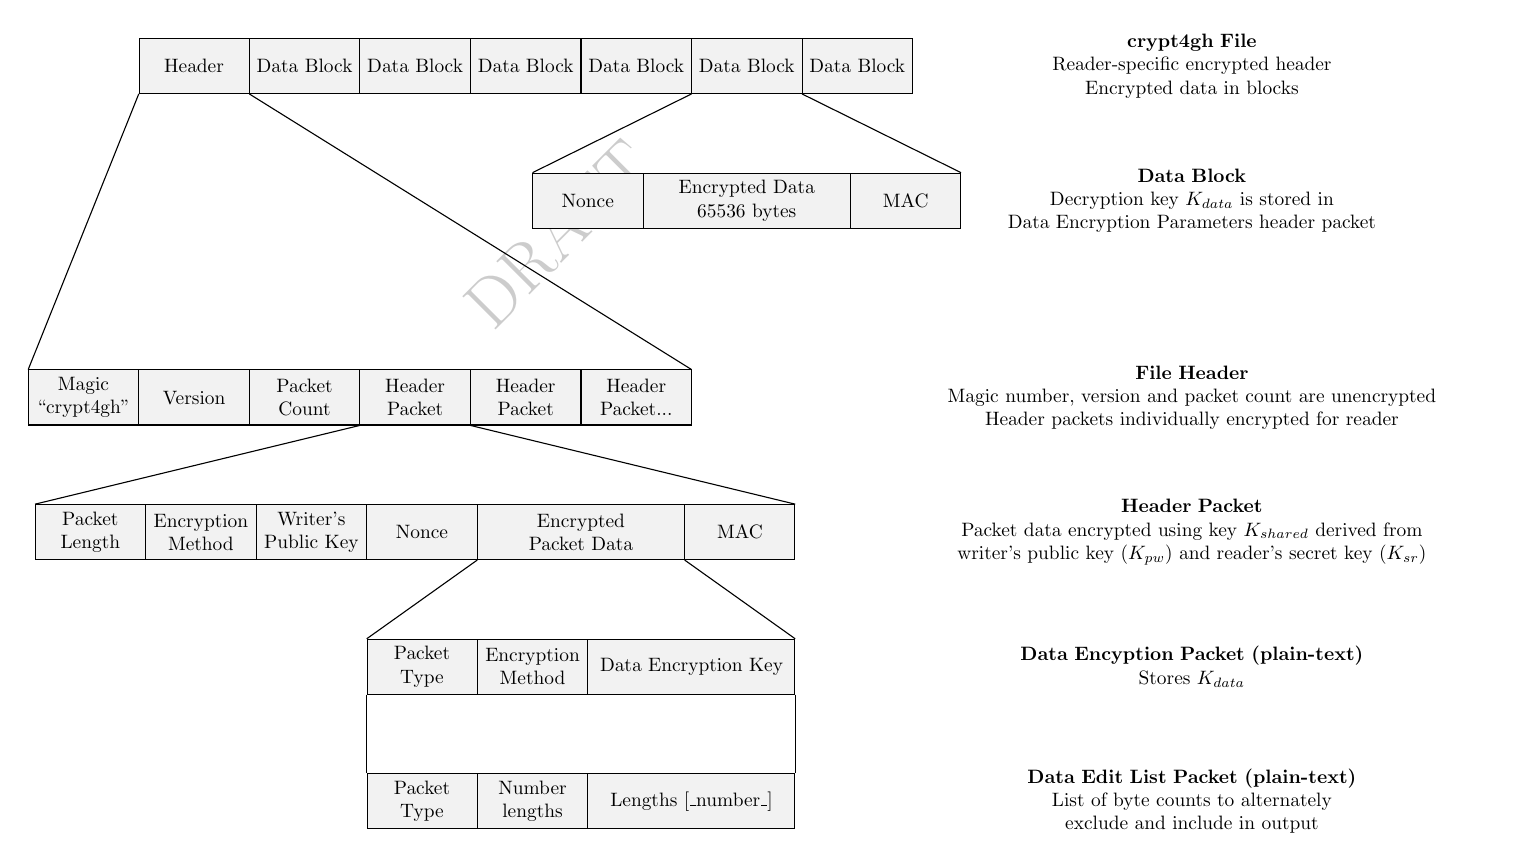
\begin{tikzpicture}[
    every node/.style={scale=0.7},
    boxes/.style={rectangle split,rectangle split parts=#1,draw,rectangle split horizontal,text width=5em,align=center,minimum height=1cm,fill=black!5,on grid},
    notes/.style={text width=20em,align=center,minimum height=1cm,on grid},
  ]
\node (file) [boxes=7] {
\nodepart{one}Header
\nodepart{two}Data Block
\nodepart{three}Data Block
\nodepart{four}Data Block
\nodepart{five}Data Block
\nodepart{six}Data Block
\nodepart{seven}Data Block
};
\node (file notes) [notes,right=of file.east] {
  \textbf{crypt4gh File} \\
  Reader-specific encrypted header \\
  Encrypted data in blocks
};

\node (data block) [boxes=3,below=1 of file.six south] {
\nodepart{one}Nonce
\nodepart[text width=10em]{two}Encrypted Data \\ 65536 bytes
\nodepart{three}MAC
};
\draw (file.five split south) to (data block.north west);
\draw (file.six split south) to (data block.north east);
\node (data block notes) at (data block -| file notes) [notes] {
  \textbf{Data Block} \\
  Decryption key $K_{data}$ is stored in \\
  Data Encryption Parameters header packet
};

\node (header) [boxes=6,below=3.5 of file.two split south] {
\nodepart{one}Magic \\ ``crypt4gh''
\nodepart{two}Version
\nodepart{three}Packet Count
\nodepart{four}Header Packet
\nodepart{five}Header Packet
\nodepart{six}Header Packet...
};
\draw (file.south west) to (header.north west);
\draw (file.one split south) to (header.north east);
\node (header notes) at (header -| file notes) [notes,text width=30em] {
  \textbf{File Header} \\
  Magic number, version and packet count are unencrypted \\
  Header packets individually encrypted for reader
};

\node (header packet) [boxes=6,below=of header.four south] {
\nodepart{one}Packet Length
\nodepart{two}Encryption Method
\nodepart{three}Writer's Public Key
\nodepart{four}Nonce
\nodepart[text width=10em]{five}Encrypted Packet Data
\nodepart{six}MAC
};
\draw (header.three split south) to (header packet.north west);
\draw (header.four split south) to (header packet.north east);
\node (header packet notes) at (header packet -| file notes) [notes,text width=30em] {
  \textbf{Header Packet} \\
  Packet data encrypted using key $K_{shared}$ derived from writer's public key ($K_{pw}$) and reader's secret key ($K_{sr}$)
};

\node (data encryption packet) [boxes=3,below=of header packet.five south] {
\nodepart{one}Packet Type
\nodepart{two}Encryption Method
\nodepart[text width=10em]{three}Data Encryption Key
};
\draw (header packet.four split south) to (data encryption packet.north west);
\draw (header packet.five split south) to (data encryption packet.north east);
\node (data encryption packet notes) at (data encryption packet -| file notes) [notes] {
  \textbf{Data Encyption Packet (plain-text)} \\
  Stores $K_{data}$
};

\node (data edit list) [boxes=3,below=of data encryption packet.south] {
\nodepart{one}Packet Type
\nodepart{two}Number lengths
\nodepart[text width=10em]{three}Lengths [\_number\_]
};
\draw (data encryption packet.south west) to (data edit list.north west);
\draw (data encryption packet.south east) to (data edit list.north east);
\node (data edit list notes) at (data edit list -| file notes) [notes] {
  \textbf{Data Edit List Packet (plain-text)} \\
  List of byte counts to alternately exclude and include in output
};
\end{tikzpicture}
\end{center}

The encrypted file structure, shown in the diagram above, consists of the following parts:

\begin{itemize}
\item A header containing: a ``magic'' string, version number and header packet count.
\begin{itemize}
\item A ``magic'' string for file type identification.
\item A version number.
\item The header packet count.
\item One or more header packets containing:
\begin{itemize}
\item The packet length in bytes.
\item The method used to encrypt the header packet data.
\item The writer's public key  ($K_{pw}$) used to encrypt the header packet data.
This is needed (along with the reader's secret key $K_{sr}$)
to calculate the shared key used to encrypt the header packet.
\item A random ``nonce'', also required for decryption.
\item The encrypted data for the header packet.
\item A MAC calculated over the encrypted header packet data.
\end{itemize}
The first item in the encrypted header packet data is a code indicating the packet type.
This is followed by type-specific data, described in section~\ref{overview:header_packet_types}.
\end{itemize}
\item The encrypted data.
This is the actual application data, stored in a sequence of blocks containing:
\begin{itemize}
\item A random ``nonce'', needed for decryption.
\item 64 kilobytes of encrypted data (the last block may contain less than this).
\item A MAC calculated over the encrypted data.
\end{itemize}
\end{itemize}

\subsection{Header Packet Types}\label{overview:header_packet_types}
There are two types of header packet:
\begin{itemize}
\item Data encryption key packets.

These describe the parameters used to encrypt one or more of the data blocks.
They contain a code indicating the type of encryption, and the symmetric key ($K_{data}$) needed to decrypt the data.

If parts of the data have been encrypted with different keys, more than one of this packet type will be present.

\item Data edit list packets.

These packets allow parts of the data to be discarded after decryption.
They can be used to avoid having to decrypt and re-encrypt files during splicing operations.

For example, a user may want to extract the blocks corresponding to Chromosome X from a CRAM file and store them
in a new file.
If the start and end points of the extract do not correspond to a 64Kbyte data block boundary, they would normally
have to decrypt all of the data blocks covering the region, discard a few bytes from the start and end, re-encrypt the
remaining data and store it in a new file.

The data edit list enables a simpler solution where the necessary encrypted data blocks are copied directly into
the new file.
On reading, the data blocks are decrypted and then the edit list is used to find out which parts of the unencrypted
data should be discarded.
\end{itemize}

\subsection{Encoding For Multiple Public/Secret Key Pairs}

It is sometimes useful to encrypt files so that they can be accessed using more than one secret key ($K_{sr}$).
For example, multiple members of a team may need to access to a file with their own key.

To allow this,
the header packet data is encrypted using each reader's public key ($K_{pr}$) and stored in a separate header packet
for each individual reader.

Where this is done, it is likely that anyone reading the file will only have the correct secret key ($K_{sr}$) for a
subset of the header packets.
Attempting to decode a header packet with the wrong key will result in a failure to verify the MAC stored in the file.
When this happens, implementations should ignore the undecodable header packet and move on to the next one.
Failing to decrypt a packet in this way SHOULD NOT cause an error to be reported;
however an error MUST be raised if, on reaching the end of the header,
it has not been possible to decrypt at least one data encryption key packet.

\section{Detailed Specification}
\subsection{Overall Conventions}
\subsubsection{Hexadecimal Numbers}
Hexadecimal values are written using the digits 0-9, and letters a-f for values 10-15.
Values are written with the most-significant digit on the left, and prefixed with "0x".

\subsubsection{Byte Ordering}
The basic data size is the byte (8 bits).
All multi-byte values are stored in least-significant byte first (``little-endian'') order.
For example, the value 1234 decimal (0x4d2) is stored as the byte stream 0xd2 0x04.

\subsubsection{Integer Types}
Integers can be either signed or unsigned.
Signed values are stored in two's complement form.

\subsubsection{Multi-byte Integer Types}
\begin{center}
\begin{tabular}{l l l l}
\hline
\textbf{Name} & \textbf{Byte Ordering} & \textbf{Integer Type} & \textbf{Size (bytes)} \\
\hline
byte & & unsigned & 1 \\
le\_int32 & little-endian & signed & 4 \\
le\_uint32 & little-endian & unsigned & 4 \\
le\_int64 & little-endian & signed & 8 \\
le\_uint64 & little-endian & unsigned & 8 \\
le\_uint96 & little-endian & unsigned & 12 \\
\end{tabular}
\end{center}

\subsubsection{Structures}
Structure types may be defined (in C-like notation) for convenience.

\begin{verbatim}
struct demo {
  byte string[8];
  le_int32 number1;
  le_uint64 number2;
};
\end{verbatim}

When structures are serialised to a file, elements are written in the given order with no padding between them.
The above structure would be written as twenty bytes - eight for the array `string', four for the integer `number1',
and eight for the integer `number2'.

\subsubsection{Enumerated Types}
Enumerated types may only take one of a given set of values.
The data type used to store the enumerated value is given in angle brackets after the type name.
Every element of an enumerated type must be assigned a value.
It is not valid to compare values between two enumerated types,
except to compare for (in)equality.

\begin{verbatim}
enum Animal<le_uint32> {
  cat    = 1;
  dog    = 2;
  rabbit = 3;
};
\end{verbatim}

\subsubsection{Variants}
Parts of structures may vary depending on information available at the time of decoding.
Which variant to use is selected by an enumerated type.
There must be a case for every possible enumerated value.
Cases have limited fall-through.
Consecutive cases with no fields in between all contain the same fields.

\begin{verbatim}
struct AnimalFeatures {
  select (enum Animal) {
    case cat:
    case dog:
      le_uint32 hairyness;
      le_uint32 whisker_length;

    case rabbit:
      le_uint32 ear_length;
  };
};
\end{verbatim}

For the `cat' and `dog' cases, `struct AnimalFeatures' is eight bytes long and contains two unsigned four-byte
little-endian values.
For the `rabbit' case it is four bytes long and contains a single four-byte little-endian value.

If the cases are different lengths (as above), then the size of the overall structure depends on the variant chosen.
There is NO padding to make the cases the same length unless it is explicitly defined.

\subsection{Header}

The file starts with a header, with the following structure:

\begin{verbatim}
struct Header {
  byte                          magic_number[8];
  le_uint32                     version;
  le_uint32                     header_packet_count;
  Encrypted_header_packet       header_packets[header_packet_count]
};
\end{verbatim}

The \kw{magic\_number} is the ASCII representation of the string ``crypt4gh''.

The version number is stored as a four-byte little-endian unsigned integer.
The current version number is 1.

The current byte representation of the magic number and version is:
\begin{verbatim}
0x63 0x72 0x79 0x70 0x74 0x34 0x67 0x68 0x01 0x00 0x00 0x00
============= magic_number============= ===== version =====
\end{verbatim}

\kw{header\_packet\_count} is the number of header packets that follow.

\subsubsection{Header Packets}\label{header:encryption}

The header packets are defined as:

\begin{verbatim}
enum Header_encryption_method<le_uint32> {
  X25519_chacha20_ietf_poly1305 = 0;
};

struct Header_packet {
  le_uint32                           packet_length;
  Header_encryption_method<le_uint32> packet_encryption;

  select (packet_encryption) {
    case X25519_chacha20_ietf_poly1305:
      byte   writer_public_key[32];
      byte   nonce[12];
  };

  byte encrypted_payload[];

  select (packet_encryption) {
    case X25519_chacha20_ietf_poly1305:
      byte MAC[16];
  };
};
\end{verbatim}

\kw{packet\_length} is the length of the entire header packet (including the \kw{packet\_length} itself).
To prevent packet types from being guessed by looking at the size, it is permitted for the \kw{packet\_length} to be
longer than strictly needed to encode all of the packet data.
Any remaining space after the actual data should be padded in a suitable manner (for example by setting it to zero)
and encrypted.

\kw{packet\_encryption} is the encryption method used for this header packet.

\kw{writer\_public\_key} ($K_{pw}$) and \kw{nonce} are parameters needed to decrypt the \kw{encrypted\_payload} in the
packet.

\kw{encrypted\_payload} is the encrypted part of the header packet, for which the plain-text is described below.

\kw{MAC} is a message authentication code calculated over the encrypted data.

Implementations should ignore any header packets that they cannot decrypt successfully, as these may have
been intended for a different reader.

\subsubsection{Header packet encrypted payload}

The \kw{encrypted\_payload} part of the header packet contains the following plain-text:

\begin{verbatim}
enum Header_packet_type<le_uint32> {
  data_encryption_parameters = 0;
  data_edit_list = 1;
};

enum Data_encryption_method<le_uint32> {
  chacha20_ietf_poly1305 = 0;
};

struct Encrypted_header_packet {
  Header_packet_type<le_uint32> packet_type;

  select (packet_type) {
    case data_encryption_parameters:
      enum Data_encryption_method<le_uint32>  data_encryption_method;
      select (data_encryption_method) {
        case chacha20_ietf_poly1305:
          byte  data_key[32];
      };

    case data_edit_list:
      le_uint32 number_lengths;
      le_uint64 lengths[number_lengths];
  };
};
\end{verbatim}

\kw{packet\_type} defines what sort of data packet this is.

\subsubsection{data\_encryption\_parameters packet}\label{header:data_encryption_parameters}

This packet contains the parameters needed to decrypt the data part of the file.

\kw{data\_encryption\_method} is an enumerated type that describes the type of encryption used.

\kw{data\_key} is the symmetric key $K_{data}$ used to decode the data section.

To allow parts of the data to be encrypted with different $K_{data}$ keys,
more than one of this packet type may be present.
If there is more than one, the \kw{data\_encryption\_method} MUST be the same for all of them to prevent problems
with random access in the encrypted file.

\subsubsection{data\_edit\_list packet}

This packet contains a list of edits that should be applied to the plain-text data following decryption.

\kw{number\_lengths} is the number of items in the \kw{lengths} array.

\kw{lengths} is an array of byte counts.

Application of the edit list to the plain-text is described in section~\ref{data:edit_list}.

It is not permitted to have more than one edit list.
If more than one edit list is present, the file SHOULD be rejected.

\subsection{Header packet encryption}

\subsubsection{X25519\_chacha20\_ietf\_poly1305 Encryption}~\label{header:X25519}

This method uses Elliptic Curve Diffie-Hellman key exchange with additional hashing to generate a shared
key ($K_{shared}$).
$K_{shared}$ is then used along with a randomly-generated nonce to encrypt the header packet data using the
ChaCha20-IETF-Poly1305 construction.
The elliptic curve algorithm used is X25519, described in section 5 of \cite{RFC7748}.

Encryption requires the writer's public and secret keys ($K_{pw}$ and $K_{sw}$), the reader's public key ($K_{pr}$)
and a nonce ($N$).

The nonce is a unique initialisation vector.
In ChaCha20-IETF-Poly1305 it is 12 bytes long.
This value MUST be unique for each packet encrypted with the same reader's and writer's keys.
The best way to ensure this is to generate a value with a cryptographically-secure random number generator.

The secret keys MUST be generated using a cryptographically-secure random number generator.
The corresponding public keys are derived using the method in section 6.1 of \cite{RFC7748}.

$K_p = X25519(K_s, 9)$

The writer's secret key and the reader's public key are used to generate a Diffie-Hellman shared key as described in
section 6.1 of \cite{RFC7748}.

$K_{dh} = X25519(K_{sw}, K_{pr})$

As the X25519 algorithm does not produce a completely uniform bit distribution,
and many possible $(K_{sw}, K_{pr})$ pairs can produce the same output,
the Diffie-Hellman key is hashed along with the two public keys to produce the final shared key.
The hash function used to do this is Blake2b, as described in \cite{RFC7693}.

$K_{shared} = Blake2b(K_{dh} || K_{pr} || K_{pw})$

As ChaCha20 uses a 32-byte key, only the first 32 bytes of $K_{shared}$ are used; the rest are discarded.

The header packet type, data and any padding is then encrypted using the method described in the
chacha20\_ietf\_poly1305 Encryption section~\ref{data:chacha20_encryption}.
Note that header packets are not segmented; they are always encrypted in a single block.

Finally, the packet length, encryption type, writer's public key $K_{pw}$,
the nonce $N$ and the encrypted header packet data are combined to make the header packet.

For extra security, writers MAY choose to discard the writer's secret key $K_{sw}$ after use.
Due to the symmetry of the Diffie-Hellman algorithm, the holder of either secret key can regenerate the shared
key as long as the other public key is known.
Deleting the writer's key $K_{sw}$ ensures only the holder of the reader's secret key $K_{sr}$ can decode the header
packet.
As long as the writer uses randomly-generated keys, it also makes accidental nonce reuse very unlikely.

\subsubsection{X25519\_chacha20\_ietf\_poly1305 Decryption}

To decrypt the header packet, the reader obtains the writer's public key $K_{pw}$ and the nonce from the beginning
of the packet.
Also needed are the reader's public and secret keys ($K_{pr}$ and $K_{sr}$).

The Diffie-Helman key is obtained using:

$K_{dh} = X25519(K_{sr}, K_{pw})$

This is then hashed to obtain the shared key (again only the first 32 bytes are retained):

$K_{shared} = Blake2b(K_{dh} || K_{pr} || K_{pw})$

The resulting key $K_{shared}$ and nonce $N$ are then used to decrypt the remainder of the packet.

If the header packet was intended for a different reader, the reader will be unable to decode the header packet
as the Poly1305 MAC will be incorrect.
This should not be considered an error.

\subsubsection{Reading the header}

The reader should check that the \kw{magic\_number} and \kw{version} in the header match the expected values.

It should then attempt to decode all of the header packets, ignoring any that do not decrypt successfully
(detected by a failure to verify the MAC).
At the end of this process the reader should have decoded at least one \kw{data\_encryption\_parameters} packet.
If no such packet was decoded, it SHOULD report an error.
If more than one is present, they should all have the same \kw{data\_encryption\_method}, otherwise the reader
SHOULD report an error.
The reader should store all of the keys that it has decoded in a list for use when decoding the encrypted data section.

If a \kw{data\_edit\_list} packet is found, the reader should store it for use while processing the data blocks.
If more than one \kw{data\_edit\_list} packet is present, the file SHOULD be rejected.

\subsection{Encrypted Data}\label{data:encryption}
\subsubsection{chacha20\_ietf\_poly1305 Encryption}\label{data:chacha20_encryption}

ChaCha20 is a stream cipher which maps a 256-bit key, nonce and counter to a 512-bit key-stream block.
In IETF mode the nonce is 96 bits long and the counter is 32 bits.
The counter starts at 1, and is incremented by 1 for each successive key-stream block.
The cipher-text is the plain-text message combined with the key-stream using the bit-wise exclusive-or operation.

Poly1305 is used to generate a 16-byte message authentication code (MAC) over the cipher-text.
As the MAC is generated over the entire cipher-text it is not possible to authenticate partially decrypted data.

ChaCha20 and Poly1305 are combined using the AEAD construction described in section 2.8 of \cite{RFC8439}.
This construction allows additional authenticated data (AAD) to be included in the Poly1305 MAC calculation.
For the purposes of this format, the AAD is zero bytes long.

\subsubsection{Segmenting the input}

To allow random access without having to authenticate the entire file, the plain-text is divided into 65536-byte
(64KiB) segments.
If the plain-text is not a multiple of 64KiB long, the last segment will be shorter.
Each segment is encrypted using the method defined in the header.
The nonce used to encrypt the segment is then stored, followed by the encrypted data, and then the MAC.

\begin{verbatim}
struct Segment {
  select (method) {
    case chacha20_ietf_poly1305:
      byte    nonce[12];
      byte[]  encrypted_data;
      byte    mac[16];
  };
};
\end{verbatim}

The addition of the \kw{nonce} and \kw{mac} bytes will expand the data slightly.
For chacha20\_ietf\_poly1305, this expansion will be 28 bytes, so a 65536 byte plain-text input will become a 65564
byte encrypted and authenticated cipher-text output.

\section{Decryption}

\subsection{chacha20\_ietf\_poly1305 Decryption}

The cipher-text is decrypted by authenticating and decrypting the segment(s) enclosing the requested byte range $[P;Q]$,
where $P<Q$.
For a range starting at position $P$, the location of the segment \kw{seg\_start} containing that position must
first be found.
For the chacha20\_ietf\_poly1305 method, when no edit list is in use, this can be done using the formula:

\begin{verbatim}
seg_start = header_len + floor(P/65536) * 65564
\end{verbatim}

For an encrypted segment starting at position \kw{seg\_start}, the nonce, then the 65536 bytes of cipher-text
(possibly fewer of it was the last segment), and finally the MAC are read.

An authentication tag is calculated over the cipher-text from that segment, and bit-wise compared to the MAC.
The cipher-text is authenticated if and only if the tags match.
If more than one key ($K_{data}$) was included in the header,
each should be tried in turn until either one authenticates correctly or no keys are left to try.
An error MUST be reported if the cipher-text is not authenticated.

The key $K_{data}$ and nonce $N$ are then used to decrypt the cipher-text for the segment, returning the plain-text.
Successive segments are decrypted, until the segment containing position $Q$ is reached.
The plain-text segments are concatenated to form the resulting output, discarding $P \mathbin{\%} 65536$ bytes from
the beginning of the first segment and retaining $Q \mathbin{\%} 65536$ bytes of the last one.

If more than one key ($K_{data}$) is in use,
readers can speed up decryption by trying the previous successful key first when attempting to authenticate each block.
However, this does open up a possible timing attack where an observer watching the decoding process can find
out where key changes occur due to the extra time needed to select the new key at these points.
If this is unacceptable, readers could either try each key for every block (although this may still be vulnerable
to timing attacks which try to detect which key was successful); or simply insist that only one key is used for
the whole file.

\subsection{Edit List}\label{data:edit_list}

The edit list is designed to assist splicing of encrypted files (for example to remove parts that are not needed
for later analysis) without having to decrypt and re-encrypt the entire file.
It is only possible to splice crypt4gh files at the 64K encryption block boundaries.
The edit list can be used to work around this limitation by describing which parts of the unencrypted blocks
should be discarded to give the final desired plain-text.

The following algorithm describes how to apply the edit list $edlist$ to unencrypted text $input$ to return
the desired edited plain-text.
In this algorithm, function \textsc{IsEmpty} returns true if a list is empty and false if not.
Function \textsc{RemoveFirst} removes the first item from a list and returns it.
\textsc{length} returns the length of a string.
\textsc{substr} returns part of a string from a given zero-based position and with a given length (or shorter if the
requested part extends beyond the end of the input string).
\textsc{StringConcatenate} returns the string concatenation of its input parameters in order from left to right.

\begin{algorithmic}[1]
\Function{ApplyEditList}{$edlist,\ input$}
\If{\Call{IsEmpty}{edlist}}
  \State \textbf{return} $input$\Comment{Trivial case with no edit list}
\EndIf
\settowidth{\maxwidth}{output}
\State \algalign{output}{\gets} ``''\Comment{Initial output is empty}
\State \algalign{pos}{\gets} $0$\Comment{Current position in the unedited plain-text}
\State \algalign{len}{\gets} \Call{length}{input}\Comment{Length of input string}
\Repeat
  \settowidth{\maxwidth}{discard}
  \State \algalign{discard}{\gets} \Call{RemoveFirst}{edlist}\Comment{Pull number of bytes to discard from list}
  \State \algalign{pos}{\gets} $pos + discard$
  \If{\Call{IsEmpty}{edlist}}
     \settowidth{\maxwidth}{output}
     \State \algalign{part}{\gets} \Call{substr}{$input, pos, len - pos$}\Comment{Append the remainder of $input$}
     \State \algalign{output}{\gets} \Call{StringConcatenate}{$output,\ part$}
  \Else
     \settowidth{\maxwidth}{output}
     \State \algalign{keep}{\gets} \Call{RemoveFirst}{edlist}\Comment{Pull number of bytes to keep from the list}
     \State \algalign{part}{\gets} \Call{substr}{$input, pos, keep$}\Comment{Append this part to $output$}
     \State \algalign{output}{\gets} \Call{StringConcatenate}{$output,\ part$}
     \State \algalign{pos}{\gets} $pos + keep$
  \EndIf
\Until{\Call{IsEmpty}{edlist}}
\State \textbf{return} $output$
\EndFunction
\end{algorithmic}

\subsubsection{Example}

Imagine that for some reason we have made an encrypted copy of ERR2436651.
\footnote{The data for this example comes from \url{ftp://ftp.sra.ebi.ac.uk/vol1/run/ERR243/ERR2436651/}.}

We would like to make a new encrypted file including just the data aligned to ChrII,
without having to decrypt and re-encrypt the desired data.
The new file will need to include the following items (note that byte ranges are zero-based inclusive):

\begin{enumerate}
\item A crypt4gh header containing the keys needed to decrypt the file.
\item The CRAM header (plain-text bytes 0 to 7852).
\item ChrII data (plain-text bytes 145110 to 453038).
\item The CRAM end-of-file block (plain-text bytes 5485074 to last byte of file at 5485111).
\end{enumerate}

None of these byte ranges align with 64K boundaries.
To avoid the need to decrypt and re-encrypt the data,
an edit list can be added to the crypt4gh header and the byte ranges are expanded to complete encrypted blocks.
After this the list of items to send will be:

\begin{enumerate}
\item A crypt4gh header containing the keys needed to decrypt the file and an edit list.
\item The CRAM header (plain-text bytes 0 to 65535).
\item ChrII data (plain-text bytes 131072 to 458751).
\item The CRAM end-of-file block (plain-text bytes 5439488 to last byte of file at 5485111).
\end{enumerate}

These segments will be concatenated to make the new file,
so in this case to obtain the desired data the edit list will contain the values:
\begin{center}
$[0, 7853, 71721, 307929, 51299, 38]$
\end{center}

Which means:

\begin{itemize}
\item Discard zero bytes from the start.
\item Keep 7853 bytes (the CRAM header).
\item Discard 57683 bytes (following the CRAM header) + 14038 bytes (before ChrII data) = 71721 bytes in total.
\item Keep 307929 bytes (ChrII data).
\item Discard 5713 bytes (following ChrII) + 45586 bytes (before the EOF block) = 51299 bytes in total.
\item Keep 38 bytes (EOF block).
This could actually be left out as it extends all the way to the end of the file.
\end{itemize}

\section{Security Considerations}
\subsection{Threat Analysis}
This format is primarily designed to protect files at rest and in transport from accidental disclosure.
Attackers are assumed to have read access to encrypted files.
Even if this is the case,
it should not be possible to decrypt the file without access to the reader's secret key ($K_{sr}$).

Some file formats use supplementary files, for example external indices.
In some cases it may be possible to deduce information about the data file from the supplementary one.
For example, it is usually trivial to determine gender from a BAM index,
and it may also be possible to detect certain other genetic conditions.
Where the main data file needs to be encrypted, such supplementary files MUST be encrypted as well.

While key management is out of scope for this document,
it should be noted that it is important that attackers are not able to access secret keys.
Implementations MUST ensure that secret keys are kept in a secure manner.

Attackers with write access to files will not be able to make changes to individual blocks as
(without access to the decryption key) they will not be able to calculate the correct MAC on the new version.
Such an attacker can, however, make block-level changes such as removing or reordering blocks.
An attacker with access to the reader's public key ($K_{pr}$) will also be able to add entire blocks by inserting a new
data\_encryption\_parameters packet in the header, and using the key stored in it to encrypt the new block.

It is expected that files using this format will be decrypted in memory for processing.
There is a risk of data being leaked either directly or through a side-channel (many of which are difficult to defend
against).
It is very likely that attackers who gain access to machines analysing data in encrypted files will be able
to make deductions about the file contents, or in the worst case either extract the entire decrypted file or
obtain the decryption keys.

Implementations SHOULD use cryptographic libraries hardened against common side-channel (e.g. timing) attacks.
Implementations MUST keep secret material as safe as possible.
For example, keys should ideally be locked into memory to avoid them being paged to a swap file.
Keys should also be securely erased as soon as they are no longer needed.
Any intermediate files written out during processing SHOULD be encrypted.

Deployments MUST take precautions to prevent attackers from accessing data while it is processed.
Note that the following list is not exhaustive.
\begin{itemize}
\item Software MUST be kept up to date for security patches.
\item Data should not be processed on machines shared by more than one user.
\item Local file systems and swap partitions should be encrypted.
\item Debugging interfaces (for example ptrace) should be disabled.
\item Machines should not be running any unnecessary processes or services.
\item Firewall rules should be used to restrict network access to only sites needed for processing the data.
\item Users should avoid running processes like web browsers that can run arbitrary code downloaded from the Internet
(even if the code is run in a sand-box environment) on a machine where encrypted data is being processed.
\end{itemize}

\subsection{Selection of Keys}
The security of the format depends on attackers not being able to guess secret keys ($K_{sr}$ and $K_{sw}$)
or the data encryption key ($K_{data}$).
The keys MUST be generated using a cryptographically-secure pseudo-random number generator.
This makes the chance of guessing a key vanishingly small.

\subsection{Nonce selection}
All header packets encrypted with the same combination of writer's secret key ($K_{sw}$)
and reader's public key ($K_{pr}$) MUST use a unique nonce.
If the writer uses the same secret key ($K_{sw}$) for more than one file then all nonces MUST be unique across all
files made with that key.
As each file will only include a few header packets this restriction can be fulfilled by generating each nonce
using a cryptographically-secure random number generator.
If the writer uses a randomly-generated $K_{sw}$ for each file, or even each header packet, the risk of nonce reuse in
the header is almost completely eliminated.

All data segments encrypted with the same key MUST use a unique nonce.
One way to ensure this is to choose a random starting point and then use a counter or linear-feedback shift
register to generate the nonce for each segment.
This method guarantees a unique value even for very long files.

For a 96-bit nonce, it may be acceptable to generate each one using a cryptographically-secure pseudo-random number
generator.
Care should be taken to ensure that the random number generator is capable of generating a long enough stream
of unique values.
Due to the birthday problem, this method will have a non-zero (but very small) probability of failing.
For example, a file of 24 Terabytes will have a reused nonce with probability of approximately $10^{-12}$

\subsection{Message Forgery}
Using ChaCha20-IETF-Poly1305 authenticates the content of each header packet and each segment of the encrypted
cipher-text.
It does not protect against the addition or removal of header packets, or the addition, removal or rearrangement
of data segments.
crypt4gh files are not signed, so there is no direct way to prove that a file was created by a given writer.

\subsection{No File Updates Permitted}
Implementations MUST NOT update encrypted files.
Once written, a section of the file must never be altered.

\bibliographystyle{abstract}

\begin{thebibliography}{XXXXXXX}

% Normative references
\subsection{Normative References}

\bibitem[RFC2119]{RFC2119}
  Bradner, S.,\\
  \emph{"Key words for use in RFCs to Indicate Requirement Levels", BCP 14, RFC 2119},\\
  \url{https://www.rfc-editor.org/info/rfc2119},\\
  March 1997

\bibitem[RFC7693]{RFC7693}
  Saarinen, M.J., Aumasson, J.P.\\
  \emph{"The BLAKE2 Cryptographic Hash and Message Authentication Code (MAC)", RFC7693},\\
  \url{https://tools.ietf.org/html/rfc7693},\\
  November 2015

\bibitem[RFC7748]{RFC7748}
  A. Langley, Google, M. Hamburg, Rambus Cryptography Research, S. Turner, sn3rd,\\
  \emph{"Elliptic Curves for Security", RFC7748},\\
  \url{https://tools.ietf.org/html/rfc7748},\\
  January 2016

\bibitem[RFC8032]{RFC8032}
  S. Josefsson, SJD AB, I. Liusvaara,\\
  \emph{"Edwards-Curve Digital Signature Algorithm (EdDSA)", RFC8032},\\
  \url{https://tools.ietf.org/html/rfc8032},\\
  January 2017

\bibitem[RFC8439]{RFC8439}
  Y. Nir, Dell EMC, A. Langley, Google, Inc.,\\
  \emph{"ChaCha20 and Poly1305 for IETF Protocols", RFC8439},\\
  \url{https://tools.ietf.org/html/rfc8439},\\
  June 2018

% Informational references
\subsection{Informational References}

\bibitem[RFC4880]{RFC4880}
  Callas, J., PGP Corporation, Donnerhacke, L., IKS GmbH, Finney, H., PGP Corporation, Shaw, D., Thayer, R.,\\
  \emph{"OpenPGP Message Format", RFC 4880},\\
  \url{https://www.rfc-editor.org/info/rfc4880},\\
  November 2007.

\bibitem[RFC8446]{RFC8446}
  Rescorla, E.,\\
  \emph{"The Transport Layer Security (TLS) Protocol Version 1.3", RFC 8446},\\
  \url{https://www.rfc-editor.org/info/rfc8446},\\
  August 2018.

\bibitem[RFC8551]{RFC8551}
  Schaad, J., August Cellars, Ramsdell, B., Brute Squad Labs, Inc., Turner, S.,\\
  \emph{"Secure/Multipurpose Internet Mail Extensions (S/MIME) Version 4.0 Message Specification", RFC 8551},\\
  \url{https://www.rfc-editor.org/info/rfc8551},\\
  April 2019.

\bibitem[AE LIMITS]{AE LIMITS}
  Luykx, A., Paterson, K.,\\
  \emph{"Limits on Authenticated Encryption Use in TLS"},\\
  \url{http://www.isg.rhul.ac.uk/~kp/TLS-AEbounds.pdf},
  August 2017.

\bibitem[Curve25519]{Curve25519}
  Bernstein, Daniel J.,\\
  \emph{"Curve25519: New Diffie-Hellman Speed Records"},\\
  \url{https://doi.org/10.1007%2F11745853_14},\\
  2006.

\bibitem[SafeCurves]{SafeCurves}
  Bernstein, Daniel J., Lange, Tanja,\\
  \emph{"SafeCurves: choosing safe curves for elliptic-curve cryptography."},\\
  \url{https://safecurves.cr.yp.to},\\
  accessed 22 July 2019.

\bibitem[Blake2]{Blake2}
  Aumasson, J-P., Neves, S., Wilcox-O’Hearn, Z., Winnerlein, C.,\\
  \emph{"BLAKE2: simpler, smaller, fast as MD5"},\\
  \url{https://eprint.iacr.org/2013/322.pdf},\\
  2013.

\bibitem[Post-Quantum]{Post-Quantum}
  Alagic, G., Alperin-Sheriff, J., Apon, D., Cooper, D., Dang, Q., Miller, C., Moody, D., Peralta, R., Perlner, R., Robinson, A., Smith-Tone, D, Liu, Y-K.,\\
  \emph{"Status Report on the First Round of the NIST Post-Quantum Cryptography Standardization Process"},\\
  \url{https://doi.org/10.6028/NIST.IR.8240},\\
  January 2019.

\bibitem[htsget]{htsget}
  Kelleher, J., Lin, M., Albach, C. H., Birney, E., Davies, R., Gourtovaia, M., Glazer, D., Gonzalez, C. Y., Jackson, D. K., Kemp, A., Marshall, J., Nowak, A., Senf, A., Tovar-Corona, J. M., Vikhorev, A., Keane, T. M., GA4GH Streaming Task Team
  \emph{"htsget: a protocol for securely streaming genomic data"}
  \url{https://doi.org/10.1093/bioinformatics/bty492}
  June 2018.

\end{thebibliography}

\appendix
\section{Rationale}

Using authenticated encryption in individual segments mirrors solutions like Transport Layer
Security (TLS) as described in~\cite{RFC8446} and prevents undetected modification of segments.
Dividing the file into fixed-size (except at the end) blocks allows random-access into the encrypted file.
The format is also designed to allow streaming reads and writes;
in particular when writing no more than 64 Kbytes of plain-text needs to be known at any point.

While the standard allows for multiple encryption methods, only one choice is currently allowed.
This simplifies implementations while allowing the current choice to be replaced in a future revision if it is found
to have any vulnerabilities.
The criteria for choosing encryption methods included having strong security guarantees, good library support
and being used in other common standards like TLS version 1.3.

\subsection{Symmetric Encryption}

For symmetric encryption, the main candidates for authenticated encryption were AES-GCM and ChaCha20-Poly1305.
Both have good security guarantees, and thanks to their use in TLS 1.3 both have good library support.
ChaCha20-Poly1305 was chosen because it allows much longer files to be encrypted.
See~\cite{AE LIMITS} for a comparison although note that our ``messages'' are $2^{16}$ bytes long,
while the figures in the paper are for $2^{14}$ bytes.

There are three common ChaCha20-Poly1305 constructions original, ChaCha20-IETF-Poly1305, and XChaCha20-Poly1305.
The main differences are the length of the nonce and the maximum message size allowed using a single nonce.
ChaCha20-IETF-Poly1305 was chosen because it has the best library support thanks to its use in Internet Engineering
Task Force protocols and the nonce length allows a very large number of messages to be encrypted under a single key.
The message length restriction of ChaCha20-IETF-Poly1305 ($64*2^{32}-64$ bytes) is not a problem as our ``messages''
are at most 64 Kbytes long.

\subsection{Public-key Algorithm}

For public-key encryption Elliptic Curve Diffie-Hellman using X25519 was chosen.
Elliptic Curve Diffie-Hellman is faster and uses smaller keys than methods such as RSA or traditional Diffie–Hellman.
X25519 is based on Curve25519 which allows fast implementations, has good security properties~\cite{Curve25519}
and has been constructed to avoid a number of possible implementation problems~\cite{SafeCurves}.
X25519 is used in TLS version 1.3, S/MIME 4.0~\cite{RFC8551} and many other protocols, and has good library support.

X25519 is used to generate a shared key.
While this key could be used on its own, its properties are not ideal because many secret/public key pairs can
generate the same key and the bit distribution across the key is not completely uniform.
To enhance the key, it is concatenated with the two public keys used in the key exchange and then passed through
a secure hash function.
The chosen hash function (Blake2b) has good library support,
is faster than SHA-2 and has similar security to that of SHA-3~\cite{Blake2}.

The generated shared key $K_{shared}$ is used as the secret material for symmetric encryption of the header packet data.
As it is already used for encrypting the data blocks, the method chosen for this is ChaCha20-IETF-Poly1305.

Like other ECDH schemes, X25519 is not resistant to attack using a quantum computer.
At the time of writing, quantum-computing resistant algorithms are undergoing standardisation~\cite{Post-Quantum}.
A future revision of this specification will add quantum-computing resistant algorithms once this process
is complete and a suitable replacement becomes widely available.

\subsection{Other Considerations}

This specification provides no way of authenticating files by signing them.
Implementing such a scheme would also involve creating infrastructure for validating the generated signatures.
This was deemed to be beyond the requirements of the format.
If authentication is required, the encrypted file can be signed separately using an existing digital signature scheme,
for example OpenPGP~\cite{RFC4880}.

Dividing the header into individually encrypted ``packets'' allows the data to be decrypted by more than one key,
and also allows parts of the data to be encrypted using different keys.
The former allows files to be accessed by more than one user without them having to share keys.
The latter allows for selective access to parts of a file - although this only works for random access.
Trying to stream such a file will likely result in an error when the reader reaches a part for which it does not have
a suitable key.

The data edit list header packets were added to make it easier to serve encrypted files using htsget~\cite{htsget}.
Htsget is designed to serve parts of a genomic data file in response to a web request,
Htsget servers return a list of file parts that should be downloaded and concatenated to give the desired result.
Most of these parts can simply be served directly from a static file store, allowing the htsget back-end to efficiently
handle a large number of requests.

Allowing htsget to serve encrypted files would be beneficial as the data in the static file store can be stored in
an encrypted form.
For efficiency (and better security),
the htsget server would want to avoid decrypting and re-encrypting the file blocks when serving them.
This is possible,
but there is a complication when the requested data does not align to the 64 Kbyte encrypted block boundaries.
The partial block would need to be rewritten so that it starts in the correct location.
As all encrypted blocks except the last must contain exactly 64 Kbytes, this would pull in data from the next block,
which would also have to be rewritten and so on until the end of the file.
This would essentially involve decrypting and re-encrypted the entire region.

A more efficient solution, which is enabled by the data edit list, is to serve the entire misaligned block and
include information about the parts that should be discarded in the header.
The client then discards the unwanted data after decryption.
Being able to serve the encrypted data directly and avoiding the need to handle plain-text should more than
compensate for the minor inefficiency of serving slightly more data (at most 131070 bytes per region) than requested.
The added complication of supporting edit lists in client code is also fairly minor compared to other
necessary parts of the format (for example key handling).

\end{document}

\title{GA4GH File Encryption Standard}
\date{\headdate}
\maketitle
\begin{quote}\small
The master version of this document can be found at
\url{https://github.com/samtools/hts-specs}.\\
This printing is version~\commitdesc\ from that repository,
last modified on the date shown above.
\end{quote}
\vspace*{1em}

\begin{abstract}
This document describes the format for Global Alliance for Genomics and Health (GA4GH) encrypted files.
Encryption helps to prevent accidental disclosure of confidential information.
Allowing programs to directly read and write data in an encrypted format reduces the chance of such disclosure.
The format described here can be used to encrypt any underlying file format.
It also allows for seeking on the encrypted data.
In particular indexes on the plain text version can also be used on the encrypted file without modification.
\end{abstract}
\newpage
\tableofcontents
\newpage
\section{Introduction}
\subsection{Purpose}
By its nature, genomic data can include information of a confidential nature about the health of individuals.
It is important that such information is not accidentally disclosed.
One part of the defence against such disclosure is to, as much as possible, keep the data in an encrypted format.

This document describes a file format that can be used to store data in an encrypted state.
Existing applications can, with minimal modification, read and write data in the encrypted format.
The choice of encryption also allows the encrypted data to be read starting from any location, facilitating indexed
access to files.

The format has the following properties:

\begin{itemize}
\item Confidentiality

Data stored in the file is only readable by holders of the correct secret decryption key.
The format does not hide the length of the encrypted file, although it is possible to pad some file structures to
obscure the length.

\item Integrity

Data is stored in a series of 64 kilobyte blocks, each of which includes a message authentication code (MAC).
Attempts to change the data in a block will make the MAC invalid; it is not possible to recalculate the MAC without
knowing the key used to encrypt the file.

The format only protects the contents of each individual block.
It does not protect against insertion, removal, or reordering of entire blocks.

\item Authentication

The format does not provide any way of authenticating files.
\end{itemize}

\subsection{Requirements}
The key words ``MUST'', ``MUST NOT'', ``REQUIRED'', ``SHALL'', ``SHALL NOT'', ``SHOULD'', ``SHOULD NOT'',
``RECOMMENDED'', ``MAY'', and ``OPTIONAL'' in this document are to be interpreted as described in \cite{RFC2119}.

\subsection{Terminology}
\begin{description}
\item[cipher-text]~\\
The encrypted version of the data.

\item[plain-text]~\\
The unencrypted version of the data.

\item[symmetric encryption]~\\
Encryption where the writer and reader use the same key.

\item[public-key encryption]~\\
Encryption where a non-secret public key is used to encrypt data and a different secret private key is used to decrypt.

\item[Elliptic-curve cryptography (ECC)]~\\
An approach to public-key cryptography based on the algebraic structure of elliptic curves over finite fields.

\item[Diffie-Hellman]~\\
A method of generating a shared cryptographic key, used for public-key encryption.

\item[Elliptic-curve Diffie-Hellman (ECDH)]~\\
A variant of Diffie-Hellman using elliptic curve cryptography.

\item[Curve25519]~\\
A widely used FIPS-140 approved ECC algorithm not encumbered by any patents \cite{RFC7748}.

\item[X25519]~\\
An elliptic-curve Diffie-Hellman algorithm using Curve25519.

\item[ChaCha20-IETF-Poly1305]~\\
ChaCha20 is a symmetric stream cipher built on a pseudo-random function that gives the advantage that one can
efficiently seek to any position in the key stream in constant time.
It is not patented.
Poly1305 is a cryptographic message authentication code (MAC).
It can be used to verify the data integrity and the authenticity of a message \cite{RFC8439}.

\item[nonce]~\\
A number that is used only once.
Such numbers are used to set the initial state in cryptographic constructions.
It is important that they are not reused as it is possible for attackers to learn information about data blocks that
have been encrypted using the same key and nonce.
In the worst case this can lead to a complete break-down of the security of the encryption.

\item[MAC]~\\
Message authentication code.
A MAC is a short tag generated by an algorithm which takes a message and a secret key as inputs.
To be secure, it should be computationally infeasible to generate the same MAC without knowing the secret key.
A holder of the secret key can run a verification algorithm on the MAC to ensure with high probability that the
message has not been altered after the MAC was generated.

\item[magic string]~\\
A byte pattern that can be used for file format identification.
Usually put at the start of a file so that software can probe the first few bytes to determine what sort of file
it is reading.

\end{description}

\section{Encrypted Format Overview}

\subsection{Keys}

A number of cryptographic keys are required by the format.
The type and function of each key is listed here,
along with symbols ($K_x$ where $_x$ is the key type) used to refer to the key in the rest of this specification.

\subsubsection{Asymmetric Keys}

This specification uses the term ``secret key'' rather than ``private key'' so that the symbol $K_s$ can be used
for secret keys and $K_p$ for public keys.

\begin{description}

\item{Reader's secret key ($K_{sr}$)}~\\
This key is used by the reader when decrypting header packets and should be kept private.
It is generated using a cryptographically-secure random number.

\item{Reader's public key ($K_{pr}$)}~\\
This key is passed to the writer so that they can encrypt header packets (section~\ref{header:encryption}) for the
reader.
It is derived from $K_{sr}$ (see section~\ref{header:X25519}).

\item{Writer's secret key ($K_{sw}$)}~\\
This key is used by the writer to encrypt header packets.
It should either be kept private, or deleted after use.
It is generated using a cryptographically-secure random number.

\item{Writer's public key ($K_{pw}$)}~\\
This key is included in the header packet (section~\ref{header:encryption}) so that the reader can use it to
derive the shared key ($K_{shared}$, see below) needed to decrypt header packet data.
It is derived from $K_{sw}$ (see section~\ref{header:X25519}).

\end{description}

\subsubsection{Symmetric keys}

\begin{description}

\item{Diffie-Hellman key ($K_{dh}$)}~\\
This is generated as part of the derivation of $K_{shared}$.

\item{Shared key ($K_{shared}$)}~\\
This key is used to encrypt header packet data.
It can be derived either from ($K_{sw}$ and $K_{pr}$) or from ($K_{sr}$ and $K_{pw}$) - see section~\ref{header:X25519}.
The writer will use the first of these derivations and the reader will use the second.

\item{Data key ($K_{data}$)}~\\
This key is used to encrypt the actual file data (section~\ref{data:encryption}).
It is generated using a cryptographically-secure random number.
The data key SHOULD be generated uniquely for each file.
This key is stored in a data\_encryption\_parameters header packet (see section~\ref{header:data_encryption_parameters}).
It is possible to encrypt parts of a file with different data keys,
in which case each key will be stored in a separate data\_encryption\_parameters header packet.

\end{description}

\subsection{File Structure}

\begin{center}
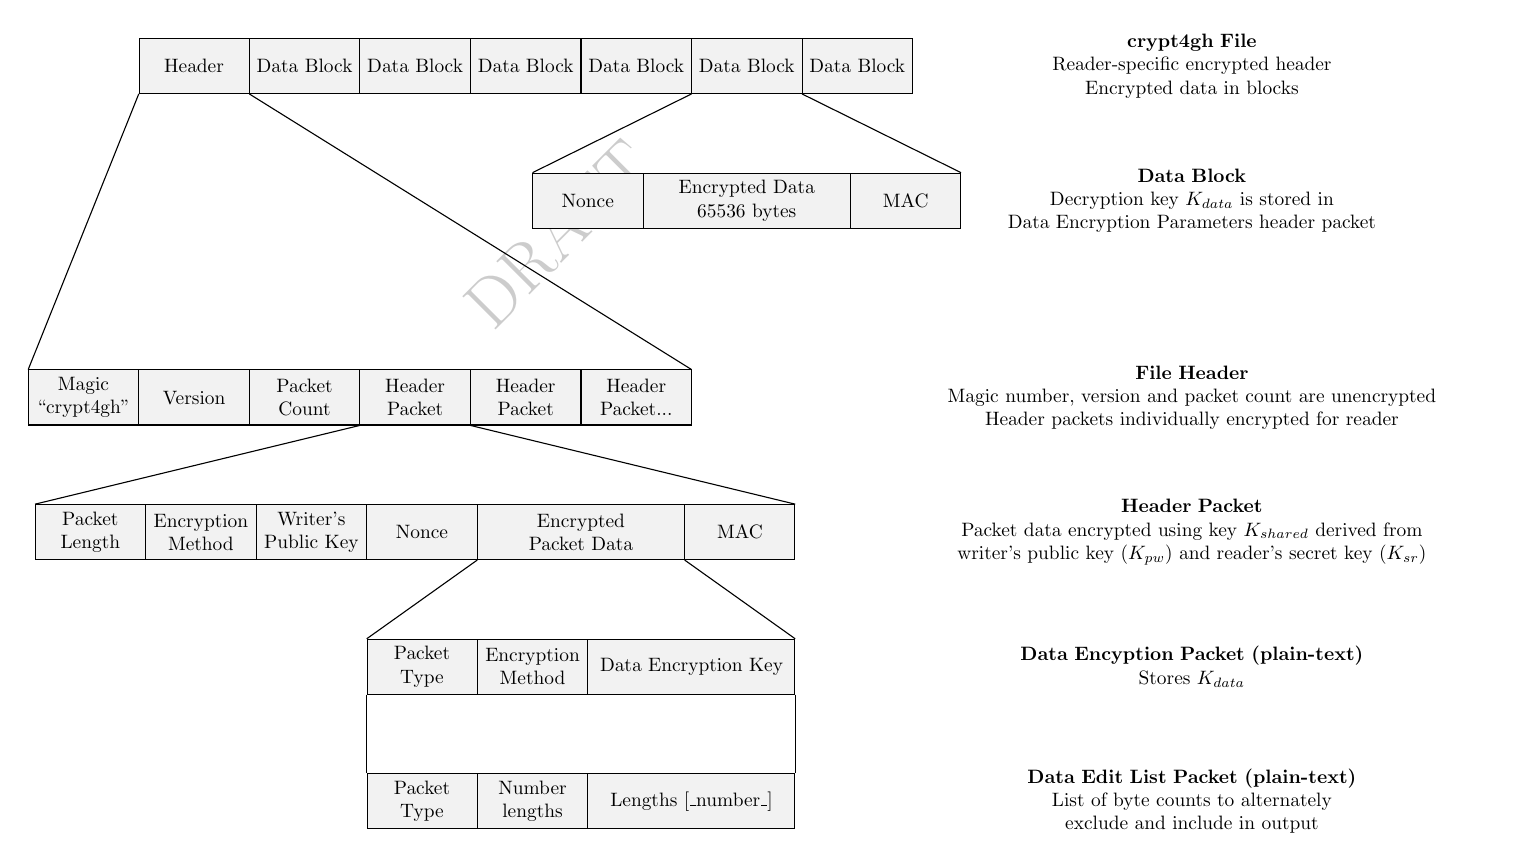
\begin{tikzpicture}[
    every node/.style={scale=0.7},
    boxes/.style={rectangle split,rectangle split parts=#1,draw,rectangle split horizontal,text width=5em,align=center,minimum height=1cm,fill=black!5,on grid},
    notes/.style={text width=20em,align=center,minimum height=1cm,on grid},
  ]
\node (file) [boxes=7] {
\nodepart{one}Header
\nodepart{two}Data Block
\nodepart{three}Data Block
\nodepart{four}Data Block
\nodepart{five}Data Block
\nodepart{six}Data Block
\nodepart{seven}Data Block
};
\node (file notes) [notes,right=of file.east] {
  \textbf{crypt4gh File} \\
  Reader-specific encrypted header \\
  Encrypted data in blocks
};

\node (data block) [boxes=3,below=1 of file.six south] {
\nodepart{one}Nonce
\nodepart[text width=10em]{two}Encrypted Data \\ 65536 bytes
\nodepart{three}MAC
};
\draw (file.five split south) to (data block.north west);
\draw (file.six split south) to (data block.north east);
\node (data block notes) at (data block -| file notes) [notes] {
  \textbf{Data Block} \\
  Decryption key $K_{data}$ is stored in \\
  Data Encryption Parameters header packet
};

\node (header) [boxes=6,below=3.5 of file.two split south] {
\nodepart{one}Magic \\ ``crypt4gh''
\nodepart{two}Version
\nodepart{three}Packet Count
\nodepart{four}Header Packet
\nodepart{five}Header Packet
\nodepart{six}Header Packet...
};
\draw (file.south west) to (header.north west);
\draw (file.one split south) to (header.north east);
\node (header notes) at (header -| file notes) [notes,text width=30em] {
  \textbf{File Header} \\
  Magic number, version and packet count are unencrypted \\
  Header packets individually encrypted for reader
};

\node (header packet) [boxes=6,below=of header.four south] {
\nodepart{one}Packet Length
\nodepart{two}Encryption Method
\nodepart{three}Writer's Public Key
\nodepart{four}Nonce
\nodepart[text width=10em]{five}Encrypted Packet Data
\nodepart{six}MAC
};
\draw (header.three split south) to (header packet.north west);
\draw (header.four split south) to (header packet.north east);
\node (header packet notes) at (header packet -| file notes) [notes,text width=30em] {
  \textbf{Header Packet} \\
  Packet data encrypted using key $K_{shared}$ derived from writer's public key ($K_{pw}$) and reader's secret key ($K_{sr}$)
};

\node (data encryption packet) [boxes=3,below=of header packet.five south] {
\nodepart{one}Packet Type
\nodepart{two}Encryption Method
\nodepart[text width=10em]{three}Data Encryption Key
};
\draw (header packet.four split south) to (data encryption packet.north west);
\draw (header packet.five split south) to (data encryption packet.north east);
\node (data encryption packet notes) at (data encryption packet -| file notes) [notes] {
  \textbf{Data Encyption Packet (plain-text)} \\
  Stores $K_{data}$
};

\node (data edit list) [boxes=3,below=of data encryption packet.south] {
\nodepart{one}Packet Type
\nodepart{two}Number lengths
\nodepart[text width=10em]{three}Lengths [\_number\_]
};
\draw (data encryption packet.south west) to (data edit list.north west);
\draw (data encryption packet.south east) to (data edit list.north east);
\node (data edit list notes) at (data edit list -| file notes) [notes] {
  \textbf{Data Edit List Packet (plain-text)} \\
  List of byte counts to alternately exclude and include in output
};
\end{tikzpicture}
\end{center}

The encrypted file structure, shown in the diagram above, consists of the following parts:

\begin{itemize}
\item A header containing: a ``magic'' string, version number and header packet count.
\begin{itemize}
\item A ``magic'' string for file type identification.
\item A version number.
\item The header packet count.
\item One or more header packets containing:
\begin{itemize}
\item The packet length in bytes.
\item The method used to encrypt the header packet data.
\item The writer's public key  ($K_{pw}$) used to encrypt the header packet data.
This is needed (along with the reader's secret key $K_{sr}$)
to calculate the shared key used to encrypt the header packet.
\item A random ``nonce'', also required for decryption.
\item The encrypted data for the header packet.
\item A MAC calculated over the encrypted header packet data.
\end{itemize}
The first item in the encrypted header packet data is a code indicating the packet type.
This is followed by type-specific data, described in section~\ref{overview:header_packet_types}.
\end{itemize}
\item The encrypted data.
This is the actual application data, stored in a sequence of blocks containing:
\begin{itemize}
\item A random ``nonce'', needed for decryption.
\item 64 kilobytes of encrypted data (the last block may contain less than this).
\item A MAC calculated over the encrypted data.
\end{itemize}
\end{itemize}

\subsection{Header Packet Types}\label{overview:header_packet_types}
There are two types of header packet:
\begin{itemize}
\item Data encryption key packets.

These describe the parameters used to encrypt one or more of the data blocks.
They contain a code indicating the type of encryption, and the symmetric key ($K_{data}$) needed to decrypt the data.

If parts of the data have been encrypted with different keys, more than one of this packet type will be present.

\item Data edit list packets.

These packets allow parts of the data to be discarded after decryption.
They can be used to avoid having to decrypt and re-encrypt files during splicing operations.

For example, a user may want to extract the blocks corresponding to Chromosome X from a CRAM file and store them
in a new file.
If the start and end points of the extract do not correspond to a 64Kbyte data block boundary, they would normally
have to decrypt all of the data blocks covering the region, discard a few bytes from the start and end, re-encrypt the
remaining data and store it in a new file.

The data edit list enables a simpler solution where the necessary encrypted data blocks are copied directly into
the new file.
On reading, the data blocks are decrypted and then the edit list is used to find out which parts of the unencrypted
data should be discarded.
\end{itemize}

\subsection{Encoding For Multiple Public/Secret Key Pairs}

It is sometimes useful to encrypt files so that they can be accessed using more than one secret key ($K_{sr}$).
For example, multiple members of a team may need to access to a file with their own key.

To allow this,
the header packet data is encrypted using each reader's public key ($K_{pr}$) and stored in a separate header packet
for each individual reader.

Where this is done, it is likely that anyone reading the file will only have the correct secret key ($K_{sr}$) for a
subset of the header packets.
Attempting to decode a header packet with the wrong key will result in a failure to verify the MAC stored in the file.
When this happens, implementations should ignore the undecodable header packet and move on to the next one.
Failing to decrypt a packet in this way SHOULD NOT cause an error to be reported;
however an error MUST be raised if, on reaching the end of the header,
it has not been possible to decrypt at least one data encryption key packet.

\section{Detailed Specification}
\subsection{Overall Conventions}
\subsubsection{Hexadecimal Numbers}
Hexadecimal values are written using the digits 0-9, and letters a-f for values 10-15.
Values are written with the most-significant digit on the left, and prefixed with "0x".

\subsubsection{Byte Ordering}
The basic data size is the byte (8 bits).
All multi-byte values are stored in least-significant byte first (``little-endian'') order.
For example, the value 1234 decimal (0x4d2) is stored as the byte stream 0xd2 0x04.

\subsubsection{Integer Types}
Integers can be either signed or unsigned.
Signed values are stored in two's complement form.

\subsubsection{Multi-byte Integer Types}
\begin{center}
\begin{tabular}{l l l l}
\hline
\textbf{Name} & \textbf{Byte Ordering} & \textbf{Integer Type} & \textbf{Size (bytes)} \\
\hline
byte & & unsigned & 1 \\
le\_int32 & little-endian & signed & 4 \\
le\_uint32 & little-endian & unsigned & 4 \\
le\_int64 & little-endian & signed & 8 \\
le\_uint64 & little-endian & unsigned & 8 \\
le\_uint96 & little-endian & unsigned & 12 \\
\end{tabular}
\end{center}

\subsubsection{Structures}
Structure types may be defined (in C-like notation) for convenience.

\begin{verbatim}
struct demo {
  byte string[8];
  le_int32 number1;
  le_uint64 number2;
};
\end{verbatim}

When structures are serialised to a file, elements are written in the given order with no padding between them.
The above structure would be written as twenty bytes - eight for the array `string', four for the integer `number1',
and eight for the integer `number2'.

\subsubsection{Enumerated Types}
Enumerated types may only take one of a given set of values.
The data type used to store the enumerated value is given in angle brackets after the type name.
Every element of an enumerated type must be assigned a value.
It is not valid to compare values between two enumerated types,
except to compare for (in)equality.

\begin{verbatim}
enum Animal<le_uint32> {
  cat    = 1;
  dog    = 2;
  rabbit = 3;
};
\end{verbatim}

\subsubsection{Variants}
Parts of structures may vary depending on information available at the time of decoding.
Which variant to use is selected by an enumerated type.
There must be a case for every possible enumerated value.
Cases have limited fall-through.
Consecutive cases with no fields in between all contain the same fields.

\begin{verbatim}
struct AnimalFeatures {
  select (enum Animal) {
    case cat:
    case dog:
      le_uint32 hairyness;
      le_uint32 whisker_length;

    case rabbit:
      le_uint32 ear_length;
  };
};
\end{verbatim}

For the `cat' and `dog' cases, `struct AnimalFeatures' is eight bytes long and contains two unsigned four-byte
little-endian values.
For the `rabbit' case it is four bytes long and contains a single four-byte little-endian value.

If the cases are different lengths (as above), then the size of the overall structure depends on the variant chosen.
There is NO padding to make the cases the same length unless it is explicitly defined.

\subsection{Header}

The file starts with a header, with the following structure:

\begin{verbatim}
struct Header {
  byte                          magic_number[8];
  le_uint32                     version;
  le_uint32                     header_packet_count;
  Encrypted_header_packet       header_packets[header_packet_count]
};
\end{verbatim}

The \kw{magic\_number} is the ASCII representation of the string ``crypt4gh''.

The version number is stored as a four-byte little-endian unsigned integer.
The current version number is 1.

The current byte representation of the magic number and version is:
\begin{verbatim}
0x63 0x72 0x79 0x70 0x74 0x34 0x67 0x68 0x01 0x00 0x00 0x00
============= magic_number============= ===== version =====
\end{verbatim}

\kw{header\_packet\_count} is the number of header packets that follow.

\subsubsection{Header Packets}\label{header:encryption}

The header packets are defined as:

\begin{verbatim}
enum Header_encryption_method<le_uint32> {
  X25519_chacha20_ietf_poly1305 = 0;
};

struct Header_packet {
  le_uint32                           packet_length;
  Header_encryption_method<le_uint32> packet_encryption;

  select (packet_encryption) {
    case X25519_chacha20_ietf_poly1305:
      byte   writer_public_key[32];
      byte   nonce[12];
  };

  byte encrypted_payload[];

  select (packet_encryption) {
    case X25519_chacha20_ietf_poly1305:
      byte MAC[16];
  };
};
\end{verbatim}

\kw{packet\_length} is the length of the entire header packet (including the \kw{packet\_length} itself).
To prevent packet types from being guessed by looking at the size, it is permitted for the \kw{packet\_length} to be
longer than strictly needed to encode all of the packet data.
Any remaining space after the actual data should be padded in a suitable manner (for example by setting it to zero)
and encrypted.

\kw{packet\_encryption} is the encryption method used for this header packet.

\kw{writer\_public\_key} ($K_{pw}$) and \kw{nonce} are parameters needed to decrypt the \kw{encrypted\_payload} in the
packet.

\kw{encrypted\_payload} is the encrypted part of the header packet, for which the plain-text is described below.

\kw{MAC} is a message authentication code calculated over the encrypted data.

Implementations should ignore any header packets that they cannot decrypt successfully, as these may have
been intended for a different reader.

\subsubsection{Header packet encrypted payload}

The \kw{encrypted\_payload} part of the header packet contains the following plain-text:

\begin{verbatim}
enum Header_packet_type<le_uint32> {
  data_encryption_parameters = 0;
  data_edit_list = 1;
};

enum Data_encryption_method<le_uint32> {
  chacha20_ietf_poly1305 = 0;
};

struct Encrypted_header_packet {
  Header_packet_type<le_uint32> packet_type;

  select (packet_type) {
    case data_encryption_parameters:
      enum Data_encryption_method<le_uint32>  data_encryption_method;
      select (data_encryption_method) {
        case chacha20_ietf_poly1305:
          byte  data_key[32];
      };

    case data_edit_list:
      le_uint32 number_lengths;
      le_uint64 lengths[number_lengths];
  };
};
\end{verbatim}

\kw{packet\_type} defines what sort of data packet this is.

\subsubsection{data\_encryption\_parameters packet}\label{header:data_encryption_parameters}

This packet contains the parameters needed to decrypt the data part of the file.

\kw{data\_encryption\_method} is an enumerated type that describes the type of encryption used.

\kw{data\_key} is the symmetric key $K_{data}$ used to decode the data section.

To allow parts of the data to be encrypted with different $K_{data}$ keys,
more than one of this packet type may be present.
If there is more than one, the \kw{data\_encryption\_method} MUST be the same for all of them to prevent problems
with random access in the encrypted file.

\subsubsection{data\_edit\_list packet}

This packet contains a list of edits that should be applied to the plain-text data following decryption.

\kw{number\_lengths} is the number of items in the \kw{lengths} array.

\kw{lengths} is an array of byte counts.

Application of the edit list to the plain-text is described in section~\ref{data:edit_list}.

It is not permitted to have more than one edit list.
If more than one edit list is present, the file SHOULD be rejected.

\subsection{Header packet encryption}

\subsubsection{X25519\_chacha20\_ietf\_poly1305 Encryption}~\label{header:X25519}

This method uses Elliptic Curve Diffie-Hellman key exchange with additional hashing to generate a shared
key ($K_{shared}$).
$K_{shared}$ is then used along with a randomly-generated nonce to encrypt the header packet data using the
ChaCha20-IETF-Poly1305 construction.
The elliptic curve algorithm used is X25519, described in section 5 of \cite{RFC7748}.

Encryption requires the writer's public and secret keys ($K_{pw}$ and $K_{sw}$), the reader's public key ($K_{pr}$)
and a nonce ($N$).

The nonce is a unique initialisation vector.
In ChaCha20-IETF-Poly1305 it is 12 bytes long.
This value MUST be unique for each packet encrypted with the same reader's and writer's keys.
The best way to ensure this is to generate a value with a cryptographically-secure random number generator.

The secret keys MUST be generated using a cryptographically-secure random number generator.
The corresponding public keys are derived using the method in section 6.1 of \cite{RFC7748}.

$K_p = X25519(K_s, 9)$

The writer's secret key and the reader's public key are used to generate a Diffie-Hellman shared key as described in
section 6.1 of \cite{RFC7748}.

$K_{dh} = X25519(K_{sw}, K_{pr})$

As the X25519 algorithm does not produce a completely uniform bit distribution,
and many possible $(K_{sw}, K_{pr})$ pairs can produce the same output,
the Diffie-Hellman key is hashed along with the two public keys to produce the final shared key.
The hash function used to do this is Blake2b, as described in \cite{RFC7693}.

$K_{shared} = Blake2b(K_{dh} || K_{pr} || K_{pw})$

As ChaCha20 uses a 32-byte key, only the first 32 bytes of $K_{shared}$ are used; the rest are discarded.

The header packet type, data and any padding is then encrypted using the method described in the
chacha20\_ietf\_poly1305 Encryption section~\ref{data:chacha20_encryption}.
Note that header packets are not segmented; they are always encrypted in a single block.

Finally, the packet length, encryption type, writer's public key $K_{pw}$,
the nonce $N$ and the encrypted header packet data are combined to make the header packet.

For extra security, writers MAY choose to discard the writer's secret key $K_{sw}$ after use.
Due to the symmetry of the Diffie-Hellman algorithm, the holder of either secret key can regenerate the shared
key as long as the other public key is known.
Deleting the writer's key $K_{sw}$ ensures only the holder of the reader's secret key $K_{sr}$ can decode the header
packet.
As long as the writer uses randomly-generated keys, it also makes accidental nonce reuse very unlikely.

\subsubsection{X25519\_chacha20\_ietf\_poly1305 Decryption}

To decrypt the header packet, the reader obtains the writer's public key $K_{pw}$ and the nonce from the beginning
of the packet.
Also needed are the reader's public and secret keys ($K_{pr}$ and $K_{sr}$).

The Diffie-Helman key is obtained using:

$K_{dh} = X25519(K_{sr}, K_{pw})$

This is then hashed to obtain the shared key (again only the first 32 bytes are retained):

$K_{shared} = Blake2b(K_{dh} || K_{pr} || K_{pw})$

The resulting key $K_{shared}$ and nonce $N$ are then used to decrypt the remainder of the packet.

If the header packet was intended for a different reader, the reader will be unable to decode the header packet
as the Poly1305 MAC will be incorrect.
This should not be considered an error.

\subsubsection{Reading the header}

The reader should check that the \kw{magic\_number} and \kw{version} in the header match the expected values.

It should then attempt to decode all of the header packets, ignoring any that do not decrypt successfully
(detected by a failure to verify the MAC).
At the end of this process the reader should have decoded at least one \kw{data\_encryption\_parameters} packet.
If no such packet was decoded, it SHOULD report an error.
If more than one is present, they should all have the same \kw{data\_encryption\_method}, otherwise the reader
SHOULD report an error.
The reader should store all of the keys that it has decoded in a list for use when decoding the encrypted data section.

If a \kw{data\_edit\_list} packet is found, the reader should store it for use while processing the data blocks.
If more than one \kw{data\_edit\_list} packet is present, the file SHOULD be rejected.

\subsection{Encrypted Data}\label{data:encryption}
\subsubsection{chacha20\_ietf\_poly1305 Encryption}\label{data:chacha20_encryption}

ChaCha20 is a stream cipher which maps a 256-bit key, nonce and counter to a 512-bit key-stream block.
In IETF mode the nonce is 96 bits long and the counter is 32 bits.
The counter starts at 1, and is incremented by 1 for each successive key-stream block.
The cipher-text is the plain-text message combined with the key-stream using the bit-wise exclusive-or operation.

Poly1305 is used to generate a 16-byte message authentication code (MAC) over the cipher-text.
As the MAC is generated over the entire cipher-text it is not possible to authenticate partially decrypted data.

ChaCha20 and Poly1305 are combined using the AEAD construction described in section 2.8 of \cite{RFC8439}.
This construction allows additional authenticated data (AAD) to be included in the Poly1305 MAC calculation.
For the purposes of this format, the AAD is zero bytes long.

\subsubsection{Segmenting the input}

To allow random access without having to authenticate the entire file, the plain-text is divided into 65536-byte
(64KiB) segments.
If the plain-text is not a multiple of 64KiB long, the last segment will be shorter.
Each segment is encrypted using the method defined in the header.
The nonce used to encrypt the segment is then stored, followed by the encrypted data, and then the MAC.

\begin{verbatim}
struct Segment {
  select (method) {
    case chacha20_ietf_poly1305:
      byte    nonce[12];
      byte[]  encrypted_data;
      byte    mac[16];
  };
};
\end{verbatim}

The addition of the \kw{nonce} and \kw{mac} bytes will expand the data slightly.
For chacha20\_ietf\_poly1305, this expansion will be 28 bytes, so a 65536 byte plain-text input will become a 65564
byte encrypted and authenticated cipher-text output.

\section{Decryption}

\subsection{chacha20\_ietf\_poly1305 Decryption}

The cipher-text is decrypted by authenticating and decrypting the segment(s) enclosing the requested byte range $[P;Q]$,
where $P<Q$.
For a range starting at position $P$, the location of the segment \kw{seg\_start} containing that position must
first be found.
For the chacha20\_ietf\_poly1305 method, when no edit list is in use, this can be done using the formula:

\begin{verbatim}
seg_start = header_len + floor(P/65536) * 65564
\end{verbatim}

For an encrypted segment starting at position \kw{seg\_start}, the nonce, then the 65536 bytes of cipher-text
(possibly fewer of it was the last segment), and finally the MAC are read.

An authentication tag is calculated over the cipher-text from that segment, and bit-wise compared to the MAC.
The cipher-text is authenticated if and only if the tags match.
If more than one key ($K_{data}$) was included in the header,
each should be tried in turn until either one authenticates correctly or no keys are left to try.
An error MUST be reported if the cipher-text is not authenticated.

The key $K_{data}$ and nonce $N$ are then used to decrypt the cipher-text for the segment, returning the plain-text.
Successive segments are decrypted, until the segment containing position $Q$ is reached.
The plain-text segments are concatenated to form the resulting output, discarding $P \mathbin{\%} 65536$ bytes from
the beginning of the first segment and retaining $Q \mathbin{\%} 65536$ bytes of the last one.

If more than one key ($K_{data}$) is in use,
readers can speed up decryption by trying the previous successful key first when attempting to authenticate each block.
However, this does open up a possible timing attack where an observer watching the decoding process can find
out where key changes occur due to the extra time needed to select the new key at these points.
If this is unacceptable, readers could either try each key for every block (although this may still be vulnerable
to timing attacks which try to detect which key was successful); or simply insist that only one key is used for
the whole file.

\subsection{Edit List}\label{data:edit_list}

The edit list is designed to assist splicing of encrypted files (for example to remove parts that are not needed
for later analysis) without having to decrypt and re-encrypt the entire file.
It is only possible to splice crypt4gh files at the 64K encryption block boundaries.
The edit list can be used to work around this limitation by describing which parts of the unencrypted blocks
should be discarded to give the final desired plain-text.

The following algorithm describes how to apply the edit list $edlist$ to unencrypted text $input$ to return
the desired edited plain-text.
In this algorithm, function \textsc{IsEmpty} returns true if a list is empty and false if not.
Function \textsc{RemoveFirst} removes the first item from a list and returns it.
\textsc{length} returns the length of a string.
\textsc{substr} returns part of a string from a given zero-based position and with a given length (or shorter if the
requested part extends beyond the end of the input string).
\textsc{StringConcatenate} returns the string concatenation of its input parameters in order from left to right.

\begin{algorithmic}[1]
\Function{ApplyEditList}{$edlist,\ input$}
\If{\Call{IsEmpty}{edlist}}
  \State \textbf{return} $input$\Comment{Trivial case with no edit list}
\EndIf
\settowidth{\maxwidth}{output}
\State \algalign{output}{\gets} ``''\Comment{Initial output is empty}
\State \algalign{pos}{\gets} $0$\Comment{Current position in the unedited plain-text}
\State \algalign{len}{\gets} \Call{length}{input}\Comment{Length of input string}
\Repeat
  \settowidth{\maxwidth}{discard}
  \State \algalign{discard}{\gets} \Call{RemoveFirst}{edlist}\Comment{Pull number of bytes to discard from list}
  \State \algalign{pos}{\gets} $pos + discard$
  \If{\Call{IsEmpty}{edlist}}
     \settowidth{\maxwidth}{output}
     \State \algalign{part}{\gets} \Call{substr}{$input, pos, len - pos$}\Comment{Append the remainder of $input$}
     \State \algalign{output}{\gets} \Call{StringConcatenate}{$output,\ part$}
  \Else
     \settowidth{\maxwidth}{output}
     \State \algalign{keep}{\gets} \Call{RemoveFirst}{edlist}\Comment{Pull number of bytes to keep from the list}
     \State \algalign{part}{\gets} \Call{substr}{$input, pos, keep$}\Comment{Append this part to $output$}
     \State \algalign{output}{\gets} \Call{StringConcatenate}{$output,\ part$}
     \State \algalign{pos}{\gets} $pos + keep$
  \EndIf
\Until{\Call{IsEmpty}{edlist}}
\State \textbf{return} $output$
\EndFunction
\end{algorithmic}

\subsubsection{Example}

Imagine that for some reason we have made an encrypted copy of ERR2436651.
\footnote{The data for this example comes from \url{ftp://ftp.sra.ebi.ac.uk/vol1/run/ERR243/ERR2436651/}.}

We would like to make a new encrypted file including just the data aligned to ChrII,
without having to decrypt and re-encrypt the desired data.
The new file will need to include the following items (note that byte ranges are zero-based inclusive):

\begin{enumerate}
\item A crypt4gh header containing the keys needed to decrypt the file.
\item The CRAM header (plain-text bytes 0 to 7852).
\item ChrII data (plain-text bytes 145110 to 453038).
\item The CRAM end-of-file block (plain-text bytes 5485074 to last byte of file at 5485111).
\end{enumerate}

None of these byte ranges align with 64K boundaries.
To avoid the need to decrypt and re-encrypt the data,
an edit list can be added to the crypt4gh header and the byte ranges are expanded to complete encrypted blocks.
After this the list of items to send will be:

\begin{enumerate}
\item A crypt4gh header containing the keys needed to decrypt the file and an edit list.
\item The CRAM header (plain-text bytes 0 to 65535).
\item ChrII data (plain-text bytes 131072 to 458751).
\item The CRAM end-of-file block (plain-text bytes 5439488 to last byte of file at 5485111).
\end{enumerate}

These segments will be concatenated to make the new file,
so in this case to obtain the desired data the edit list will contain the values:
\begin{center}
$[0, 7853, 71721, 307929, 51299, 38]$
\end{center}

Which means:

\begin{itemize}
\item Discard zero bytes from the start.
\item Keep 7853 bytes (the CRAM header).
\item Discard 57683 bytes (following the CRAM header) + 14038 bytes (before ChrII data) = 71721 bytes in total.
\item Keep 307929 bytes (ChrII data).
\item Discard 5713 bytes (following ChrII) + 45586 bytes (before the EOF block) = 51299 bytes in total.
\item Keep 38 bytes (EOF block).
This could actually be left out as it extends all the way to the end of the file.
\end{itemize}

\section{Security Considerations}
\subsection{Threat Analysis}
This format is primarily designed to protect files at rest and in transport from accidental disclosure.
Attackers are assumed to have read access to encrypted files.
Even if this is the case,
it should not be possible to decrypt the file without access to the reader's secret key ($K_{sr}$).

Some file formats use supplementary files, for example external indices.
In some cases it may be possible to deduce information about the data file from the supplementary one.
For example, it is usually trivial to determine gender from a BAM index,
and it may also be possible to detect certain other genetic conditions.
Where the main data file needs to be encrypted, such supplementary files MUST be encrypted as well.

While key management is out of scope for this document,
it should be noted that it is important that attackers are not able to access secret keys.
Implementations MUST ensure that secret keys are kept in a secure manner.

Attackers with write access to files will not be able to make changes to individual blocks as
(without access to the decryption key) they will not be able to calculate the correct MAC on the new version.
Such an attacker can, however, make block-level changes such as removing or reordering blocks.
An attacker with access to the reader's public key ($K_{pr}$) will also be able to add entire blocks by inserting a new
data\_encryption\_parameters packet in the header, and using the key stored in it to encrypt the new block.

It is expected that files using this format will be decrypted in memory for processing.
There is a risk of data being leaked either directly or through a side-channel (many of which are difficult to defend
against).
It is very likely that attackers who gain access to machines analysing data in encrypted files will be able
to make deductions about the file contents, or in the worst case either extract the entire decrypted file or
obtain the decryption keys.

Implementations SHOULD use cryptographic libraries hardened against common side-channel (e.g. timing) attacks.
Implementations MUST keep secret material as safe as possible.
For example, keys should ideally be locked into memory to avoid them being paged to a swap file.
Keys should also be securely erased as soon as they are no longer needed.
Any intermediate files written out during processing SHOULD be encrypted.

Deployments MUST take precautions to prevent attackers from accessing data while it is processed.
Note that the following list is not exhaustive.
\begin{itemize}
\item Software MUST be kept up to date for security patches.
\item Data should not be processed on machines shared by more than one user.
\item Local file systems and swap partitions should be encrypted.
\item Debugging interfaces (for example ptrace) should be disabled.
\item Machines should not be running any unnecessary processes or services.
\item Firewall rules should be used to restrict network access to only sites needed for processing the data.
\item Users should avoid running processes like web browsers that can run arbitrary code downloaded from the Internet
(even if the code is run in a sand-box environment) on a machine where encrypted data is being processed.
\end{itemize}

\subsection{Selection of Keys}
The security of the format depends on attackers not being able to guess secret keys ($K_{sr}$ and $K_{sw}$)
or the data encryption key ($K_{data}$).
The keys MUST be generated using a cryptographically-secure pseudo-random number generator.
This makes the chance of guessing a key vanishingly small.

\subsection{Nonce selection}
All header packets encrypted with the same combination of writer's secret key ($K_{sw}$)
and reader's public key ($K_{pr}$) MUST use a unique nonce.
If the writer uses the same secret key ($K_{sw}$) for more than one file then all nonces MUST be unique across all
files made with that key.
As each file will only include a few header packets this restriction can be fulfilled by generating each nonce
using a cryptographically-secure random number generator.
If the writer uses a randomly-generated $K_{sw}$ for each file, or even each header packet, the risk of nonce reuse in
the header is almost completely eliminated.

All data segments encrypted with the same key MUST use a unique nonce.
One way to ensure this is to choose a random starting point and then use a counter or linear-feedback shift
register to generate the nonce for each segment.
This method guarantees a unique value even for very long files.

For a 96-bit nonce, it may be acceptable to generate each one using a cryptographically-secure pseudo-random number
generator.
Care should be taken to ensure that the random number generator is capable of generating a long enough stream
of unique values.
Due to the birthday problem, this method will have a non-zero (but very small) probability of failing.
For example, a file of 24 Terabytes will have a reused nonce with probability of approximately $10^{-12}$

\subsection{Message Forgery}
Using ChaCha20-IETF-Poly1305 authenticates the content of each header packet and each segment of the encrypted
cipher-text.
It does not protect against the addition or removal of header packets, or the addition, removal or rearrangement
of data segments.
crypt4gh files are not signed, so there is no direct way to prove that a file was created by a given writer.

\subsection{No File Updates Permitted}
Implementations MUST NOT update encrypted files.
Once written, a section of the file must never be altered.

\bibliographystyle{abstract}

\begin{thebibliography}{XXXXXXX}

% Normative references
\subsection{Normative References}

\bibitem[RFC2119]{RFC2119}
  Bradner, S.,\\
  \emph{"Key words for use in RFCs to Indicate Requirement Levels", BCP 14, RFC 2119},\\
  \url{https://www.rfc-editor.org/info/rfc2119},\\
  March 1997

\bibitem[RFC7693]{RFC7693}
  Saarinen, M.J., Aumasson, J.P.\\
  \emph{"The BLAKE2 Cryptographic Hash and Message Authentication Code (MAC)", RFC7693},\\
  \url{https://tools.ietf.org/html/rfc7693},\\
  November 2015

\bibitem[RFC7748]{RFC7748}
  A. Langley, Google, M. Hamburg, Rambus Cryptography Research, S. Turner, sn3rd,\\
  \emph{"Elliptic Curves for Security", RFC7748},\\
  \url{https://tools.ietf.org/html/rfc7748},\\
  January 2016

\bibitem[RFC8032]{RFC8032}
  S. Josefsson, SJD AB, I. Liusvaara,\\
  \emph{"Edwards-Curve Digital Signature Algorithm (EdDSA)", RFC8032},\\
  \url{https://tools.ietf.org/html/rfc8032},\\
  January 2017

\bibitem[RFC8439]{RFC8439}
  Y. Nir, Dell EMC, A. Langley, Google, Inc.,\\
  \emph{"ChaCha20 and Poly1305 for IETF Protocols", RFC8439},\\
  \url{https://tools.ietf.org/html/rfc8439},\\
  June 2018

% Informational references
\subsection{Informational References}

\bibitem[RFC4880]{RFC4880}
  Callas, J., PGP Corporation, Donnerhacke, L., IKS GmbH, Finney, H., PGP Corporation, Shaw, D., Thayer, R.,\\
  \emph{"OpenPGP Message Format", RFC 4880},\\
  \url{https://www.rfc-editor.org/info/rfc4880},\\
  November 2007.

\bibitem[RFC8446]{RFC8446}
  Rescorla, E.,\\
  \emph{"The Transport Layer Security (TLS) Protocol Version 1.3", RFC 8446},\\
  \url{https://www.rfc-editor.org/info/rfc8446},\\
  August 2018.

\bibitem[RFC8551]{RFC8551}
  Schaad, J., August Cellars, Ramsdell, B., Brute Squad Labs, Inc., Turner, S.,\\
  \emph{"Secure/Multipurpose Internet Mail Extensions (S/MIME) Version 4.0 Message Specification", RFC 8551},\\
  \url{https://www.rfc-editor.org/info/rfc8551},\\
  April 2019.

\bibitem[AE LIMITS]{AE LIMITS}
  Luykx, A., Paterson, K.,\\
  \emph{"Limits on Authenticated Encryption Use in TLS"},\\
  \url{http://www.isg.rhul.ac.uk/~kp/TLS-AEbounds.pdf},
  August 2017.

\bibitem[Curve25519]{Curve25519}
  Bernstein, Daniel J.,\\
  \emph{"Curve25519: New Diffie-Hellman Speed Records"},\\
  \url{https://doi.org/10.1007%2F11745853_14},\\
  2006.

\bibitem[SafeCurves]{SafeCurves}
  Bernstein, Daniel J., Lange, Tanja,\\
  \emph{"SafeCurves: choosing safe curves for elliptic-curve cryptography."},\\
  \url{https://safecurves.cr.yp.to},\\
  accessed 22 July 2019.

\bibitem[Blake2]{Blake2}
  Aumasson, J-P., Neves, S., Wilcox-O’Hearn, Z., Winnerlein, C.,\\
  \emph{"BLAKE2: simpler, smaller, fast as MD5"},\\
  \url{https://eprint.iacr.org/2013/322.pdf},\\
  2013.

\bibitem[Post-Quantum]{Post-Quantum}
  Alagic, G., Alperin-Sheriff, J., Apon, D., Cooper, D., Dang, Q., Miller, C., Moody, D., Peralta, R., Perlner, R., Robinson, A., Smith-Tone, D, Liu, Y-K.,\\
  \emph{"Status Report on the First Round of the NIST Post-Quantum Cryptography Standardization Process"},\\
  \url{https://doi.org/10.6028/NIST.IR.8240},\\
  January 2019.

\bibitem[htsget]{htsget}
  Kelleher, J., Lin, M., Albach, C. H., Birney, E., Davies, R., Gourtovaia, M., Glazer, D., Gonzalez, C. Y., Jackson, D. K., Kemp, A., Marshall, J., Nowak, A., Senf, A., Tovar-Corona, J. M., Vikhorev, A., Keane, T. M., GA4GH Streaming Task Team
  \emph{"htsget: a protocol for securely streaming genomic data"}
  \url{https://doi.org/10.1093/bioinformatics/bty492}
  June 2018.

\end{thebibliography}

\appendix
\section{Rationale}

Using authenticated encryption in individual segments mirrors solutions like Transport Layer
Security (TLS) as described in~\cite{RFC8446} and prevents undetected modification of segments.
Dividing the file into fixed-size (except at the end) blocks allows random-access into the encrypted file.
The format is also designed to allow streaming reads and writes;
in particular when writing no more than 64 Kbytes of plain-text needs to be known at any point.

While the standard allows for multiple encryption methods, only one choice is currently allowed.
This simplifies implementations while allowing the current choice to be replaced in a future revision if it is found
to have any vulnerabilities.
The criteria for choosing encryption methods included having strong security guarantees, good library support
and being used in other common standards like TLS version 1.3.

\subsection{Symmetric Encryption}

For symmetric encryption, the main candidates for authenticated encryption were AES-GCM and ChaCha20-Poly1305.
Both have good security guarantees, and thanks to their use in TLS 1.3 both have good library support.
ChaCha20-Poly1305 was chosen because it allows much longer files to be encrypted.
See~\cite{AE LIMITS} for a comparison although note that our ``messages'' are $2^{16}$ bytes long,
while the figures in the paper are for $2^{14}$ bytes.

There are three common ChaCha20-Poly1305 constructions original, ChaCha20-IETF-Poly1305, and XChaCha20-Poly1305.
The main differences are the length of the nonce and the maximum message size allowed using a single nonce.
ChaCha20-IETF-Poly1305 was chosen because it has the best library support thanks to its use in Internet Engineering
Task Force protocols and the nonce length allows a very large number of messages to be encrypted under a single key.
The message length restriction of ChaCha20-IETF-Poly1305 ($64*2^{32}-64$ bytes) is not a problem as our ``messages''
are at most 64 Kbytes long.

\subsection{Public-key Algorithm}

For public-key encryption Elliptic Curve Diffie-Hellman using X25519 was chosen.
Elliptic Curve Diffie-Hellman is faster and uses smaller keys than methods such as RSA or traditional Diffie–Hellman.
X25519 is based on Curve25519 which allows fast implementations, has good security properties~\cite{Curve25519}
and has been constructed to avoid a number of possible implementation problems~\cite{SafeCurves}.
X25519 is used in TLS version 1.3, S/MIME 4.0~\cite{RFC8551} and many other protocols, and has good library support.

X25519 is used to generate a shared key.
While this key could be used on its own, its properties are not ideal because many secret/public key pairs can
generate the same key and the bit distribution across the key is not completely uniform.
To enhance the key, it is concatenated with the two public keys used in the key exchange and then passed through
a secure hash function.
The chosen hash function (Blake2b) has good library support,
is faster than SHA-2 and has similar security to that of SHA-3~\cite{Blake2}.

The generated shared key $K_{shared}$ is used as the secret material for symmetric encryption of the header packet data.
As it is already used for encrypting the data blocks, the method chosen for this is ChaCha20-IETF-Poly1305.

Like other ECDH schemes, X25519 is not resistant to attack using a quantum computer.
At the time of writing, quantum-computing resistant algorithms are undergoing standardisation~\cite{Post-Quantum}.
A future revision of this specification will add quantum-computing resistant algorithms once this process
is complete and a suitable replacement becomes widely available.

\subsection{Other Considerations}

This specification provides no way of authenticating files by signing them.
Implementing such a scheme would also involve creating infrastructure for validating the generated signatures.
This was deemed to be beyond the requirements of the format.
If authentication is required, the encrypted file can be signed separately using an existing digital signature scheme,
for example OpenPGP~\cite{RFC4880}.

Dividing the header into individually encrypted ``packets'' allows the data to be decrypted by more than one key,
and also allows parts of the data to be encrypted using different keys.
The former allows files to be accessed by more than one user without them having to share keys.
The latter allows for selective access to parts of a file - although this only works for random access.
Trying to stream such a file will likely result in an error when the reader reaches a part for which it does not have
a suitable key.

The data edit list header packets were added to make it easier to serve encrypted files using htsget~\cite{htsget}.
Htsget is designed to serve parts of a genomic data file in response to a web request,
Htsget servers return a list of file parts that should be downloaded and concatenated to give the desired result.
Most of these parts can simply be served directly from a static file store, allowing the htsget back-end to efficiently
handle a large number of requests.

Allowing htsget to serve encrypted files would be beneficial as the data in the static file store can be stored in
an encrypted form.
For efficiency (and better security),
the htsget server would want to avoid decrypting and re-encrypting the file blocks when serving them.
This is possible,
but there is a complication when the requested data does not align to the 64 Kbyte encrypted block boundaries.
The partial block would need to be rewritten so that it starts in the correct location.
As all encrypted blocks except the last must contain exactly 64 Kbytes, this would pull in data from the next block,
which would also have to be rewritten and so on until the end of the file.
This would essentially involve decrypting and re-encrypted the entire region.

A more efficient solution, which is enabled by the data edit list, is to serve the entire misaligned block and
include information about the parts that should be discarded in the header.
The client then discards the unwanted data after decryption.
Being able to serve the encrypted data directly and avoiding the need to handle plain-text should more than
compensate for the minor inefficiency of serving slightly more data (at most 131070 bytes per region) than requested.
The added complication of supporting edit lists in client code is also fairly minor compared to other
necessary parts of the format (for example key handling).

\end{document}
